% Copyright (c) 2014,2016 Casper Ti. Vector
% Public domain.

\chapter{引言}\label{chap:1}
\section{太阳及M矮星爆发活动简介}
太阳(\textit{Sun})是距离地球最近的一颗恒星,其质量大约为$1.99\times10^{33}$ g,半径约为$6.96\times10^{10}$ cm, 距地球平均距离为$1.496\times10^{13}$ cm\parencite{Stix2004}。从光谱型来看,太阳是一颗G2V型主序星,亮度为$3.844\times10^{33}\ \mathrm{erg}\ \mathrm{s}^{-1}$。其是太阳系行星际空间中等离子体和磁场的起源\parencite{Tu1988},对地球空间环境也有相当大的影响。笼统地来说,这些磁场结构的不稳定性和变化会引起巨大的能量释放,被称为太阳上的爆发活动\parencite{Stix2004}。这些释放的能量往往以不同的形式表现出来,如加速粒子、推动物质运动和产生从$\gamma$射线直到射电波段的电磁辐射增强等\parencite{Stix2004}。

M矮星(\textit{M dwarf},或红矮星,\textit{red dwarf})是在Hertzsprung-Russell图(\textit{HR diagram})上有别于太阳(G型主序星)的另一类恒星。相比于G型主序星,它们在HR图上显示出更低的表面温度(更红)和更小的亮度。由于表面温度较低,M矮星在可见光谱上不再有像G型星一样明显的H,Ca \textsc{ii}等线。它们在可见光波段主要的光谱特征来自于一些氧化物,尤其是TiO的谱线\parencite{pols2011}。事实上,它们的质量比太阳更小,大约只有$0.08-0.50M_{\odot}$,是能够在内部维持氢核聚变的最小质量的恒星。根据Schwarzchild对流判据,整颗星的大气处于完全对流状态。\textcite{Johns-Krull1996}利用Zeeman效应发现M矮星表面有较强的磁场,大约为2-4 kG,预示着M矮星上应该有剧烈的磁活动。

下面我将对本文中关心的太阳爆发活动和M矮星上的恒星活动做一个简单介绍。
\subsection{太阳耀斑}
太阳耀斑(\textit{Solar flares})是太阳上最常见,也最容易在地面观测到的一种爆发活动。早期通常是在形成在色球H$\alpha$波段的滤光器中观测到的增亮现象,因此也被称为色球爆发(\textit{chromospheric eruption}, \cites{Lin2000})。一般来说,太阳耀斑包含一个快速的增亮过程(\textit{impulsive phase})和一个持续约为30分钟至1小时的缓慢衰减过程(\textit{Decay phase}, \cite{Stix2004})。大量的日冕磁场能量($10^{29}-10^{32}$ erg)在极短的时间内被释放,伴随着高能非热粒子的加速和低层大气的加热。随着观测的不断进步,耀斑这种爆发活动在越来越多的电磁辐射波段上被观测到(见图\ref{fig:1}),从$\gamma$射线一直延伸到射电波段\parencite{Dulk1985,Masuda1994,Thompson1995}。
\begin{figure}
	\centering
	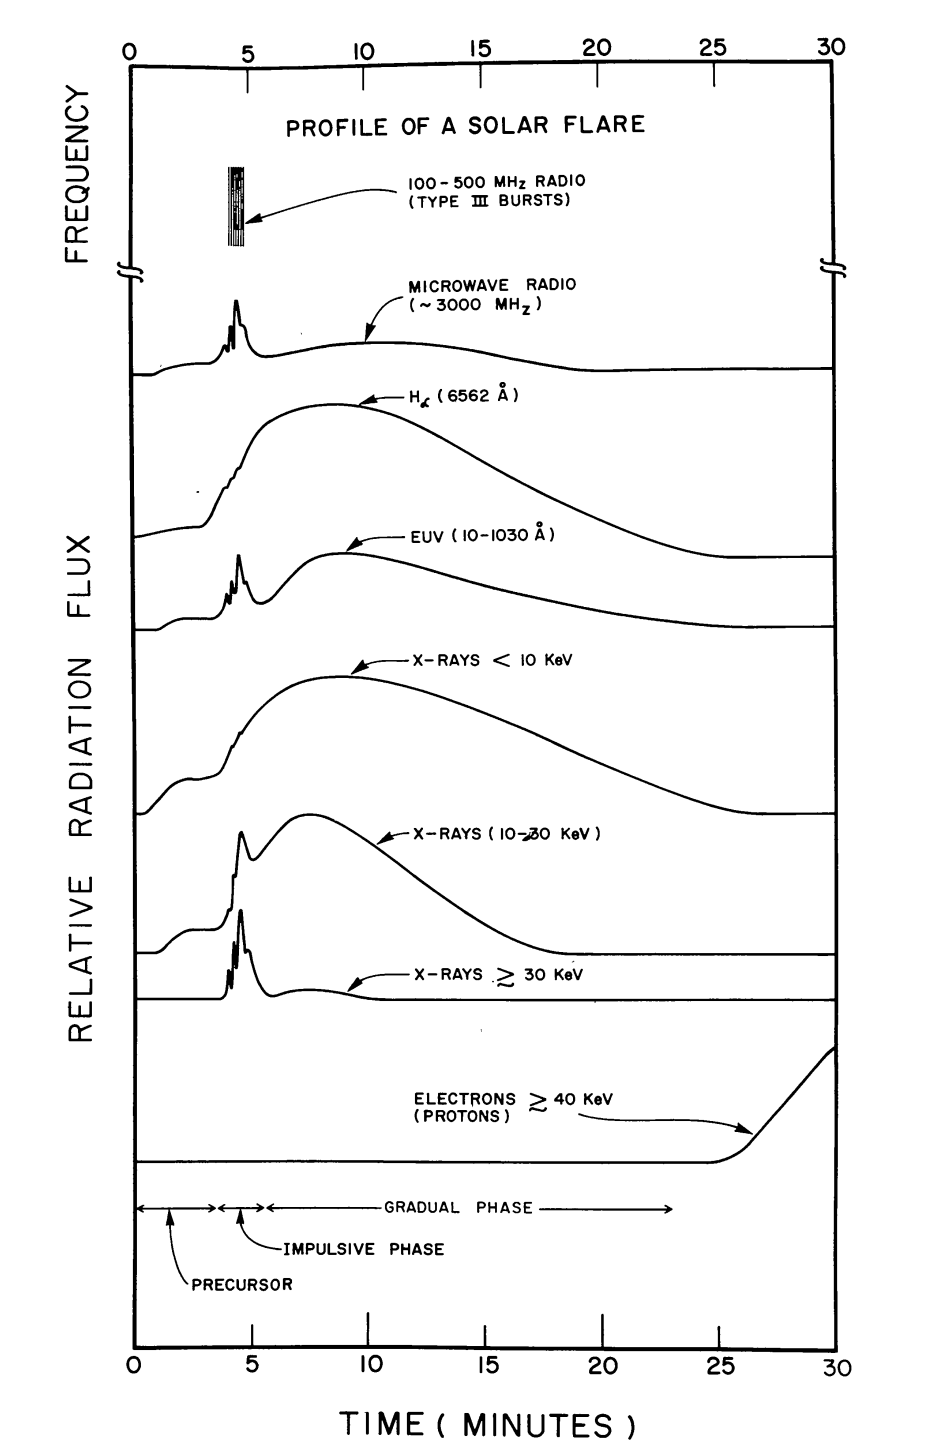
\includegraphics[width=0.4\linewidth]{figs/fig1}
	\caption{一个太阳耀斑在爆发相多波段电磁辐射变化图。来源: \textcite{Kane1974}}
	\label{fig:1}
\end{figure}



根据经典的二维CSHKP耀斑模型\parencite{Carmichael1964,Sturrock1966,Hirayama1974,Kopp1976}(见图\ref{fig:2})磁重联(\textit{magnetic reconnection})过程一般爆发在一对反向平行日冕磁感线形成的纤细的电流片中,并激发MHD激波\parencite{Shibata2011}。上方重联形成的磁感线可能携带着磁绳(\textit{flux rope})结构抛射而称为其他太阳活动(日冕物质抛射)的一部分。而下方的磁感线则连接形成了耀斑后环(\textit{post-flare loops}),这些环一般在软X射线(\textit{Soft X-ray, SXR}: $E<10$ KeV)波段被观测到,因而也被称为SXR环\parencite{Tsuneta1997,Zarro1999}。释放的日冕磁能加速了局地非热电子\parencite{Hudson2001,Tomczak2001,Krucker2007}。近期的射电观测也指出一部分电子可能被位于耀斑后环环顶的终止激波(\textit{termination shock})加速\parencite{Chen2015}。在耀斑环顶有一个硬X射线(\textit{Hard X-ray, HXR}: $E>10$ KeV)源\parencite{Masuda1994},一般认为可能来自一个高速喷流(\textit{jet})和环顶物质发生碰撞的过程\parencite{Shibata2011}。这些被加热的非热电子沿着磁感线向低层大气传播,轰击并加热低层大气。被迅速加热的色球(\textit{chromosphere})和过渡区(\textit{transition region, TR})大气产生了复杂的动力学与热力学效应。加热导致的压强增大推动一部分物质向上运动,被称为色球蒸发(\textit{chromospheric evaporation}, \cite{Fisher1985a,Fisher1985b,Fisher1985c}),这些高温等离子体填充了耀斑后环,产生了SXR辐射。在较大的色球蒸发过程当中,伴随着上百km$\ \mathrm{s}^{-1}$的物质上流\parencite{Milligan2006b},还会出现数十至上百km$\ \mathrm{s}^{-1}$的冷且致密的物质下流,被称为色球凝聚(\textit{chromospheric condensation}, \cite{Milligan2006a})。色球凝聚对一些色球谱线轮廓特征,如Mg \textsc{ii},Si \textsc{iv},和C \textsc{ii}的红翼不对称性的形成起了重要作用\parencites{Tian2015}。非热电子与致密的局地大气碰撞,在环的足点上产生了HXR辐射。加热的足点处色球和过渡区大气使的一系列形成与这些区域的谱线与连续谱辐射增强,这些位置也被称为耀斑带(\textit{flare ribbon})。具体增强的谱线有Balmer线系,Ca \textsc{ii}, Mg \textsc{ii}, C \textsc{ii}, Si \textsc{iv}, C \textsc{iv}等\parencite{Liu2015, Tian2015, Tian2018},如图\ref{fig:3}。其中一些的轮廓还出现了相当大的变化,如红蓝移,不对称性等\parencite{Li2015, Tei2018}。这些谱线的轮廓特征是我们理解太阳耀斑过程中的低层大气的演化过程的重要观测来源。

\begin{figure}
	\centering
	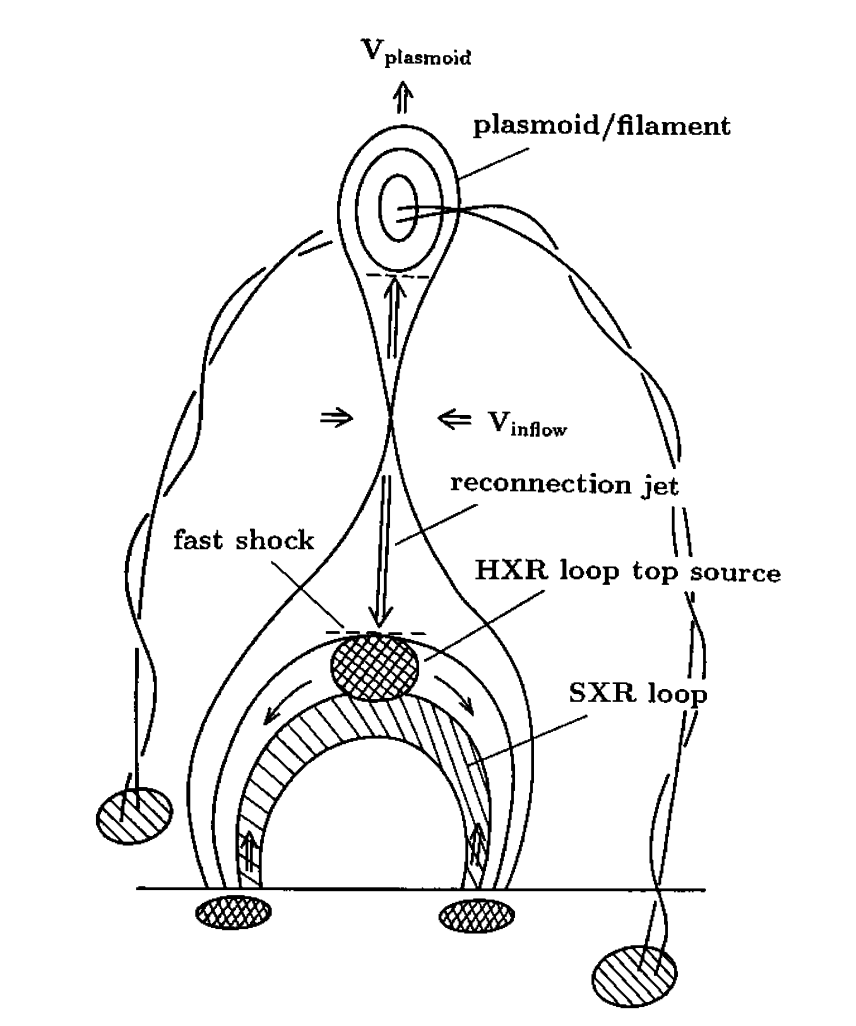
\includegraphics[width=0.5\linewidth]{figs/fig2}
	\caption{经典的二维CSHKP标准耀斑模型卡通图,加入了\textit{Yohkoh}卫星观测的新特征。来源:\textcite{Shibata1995}}
	\label{fig:2}
\end{figure}

\begin{figure}
	\centering
	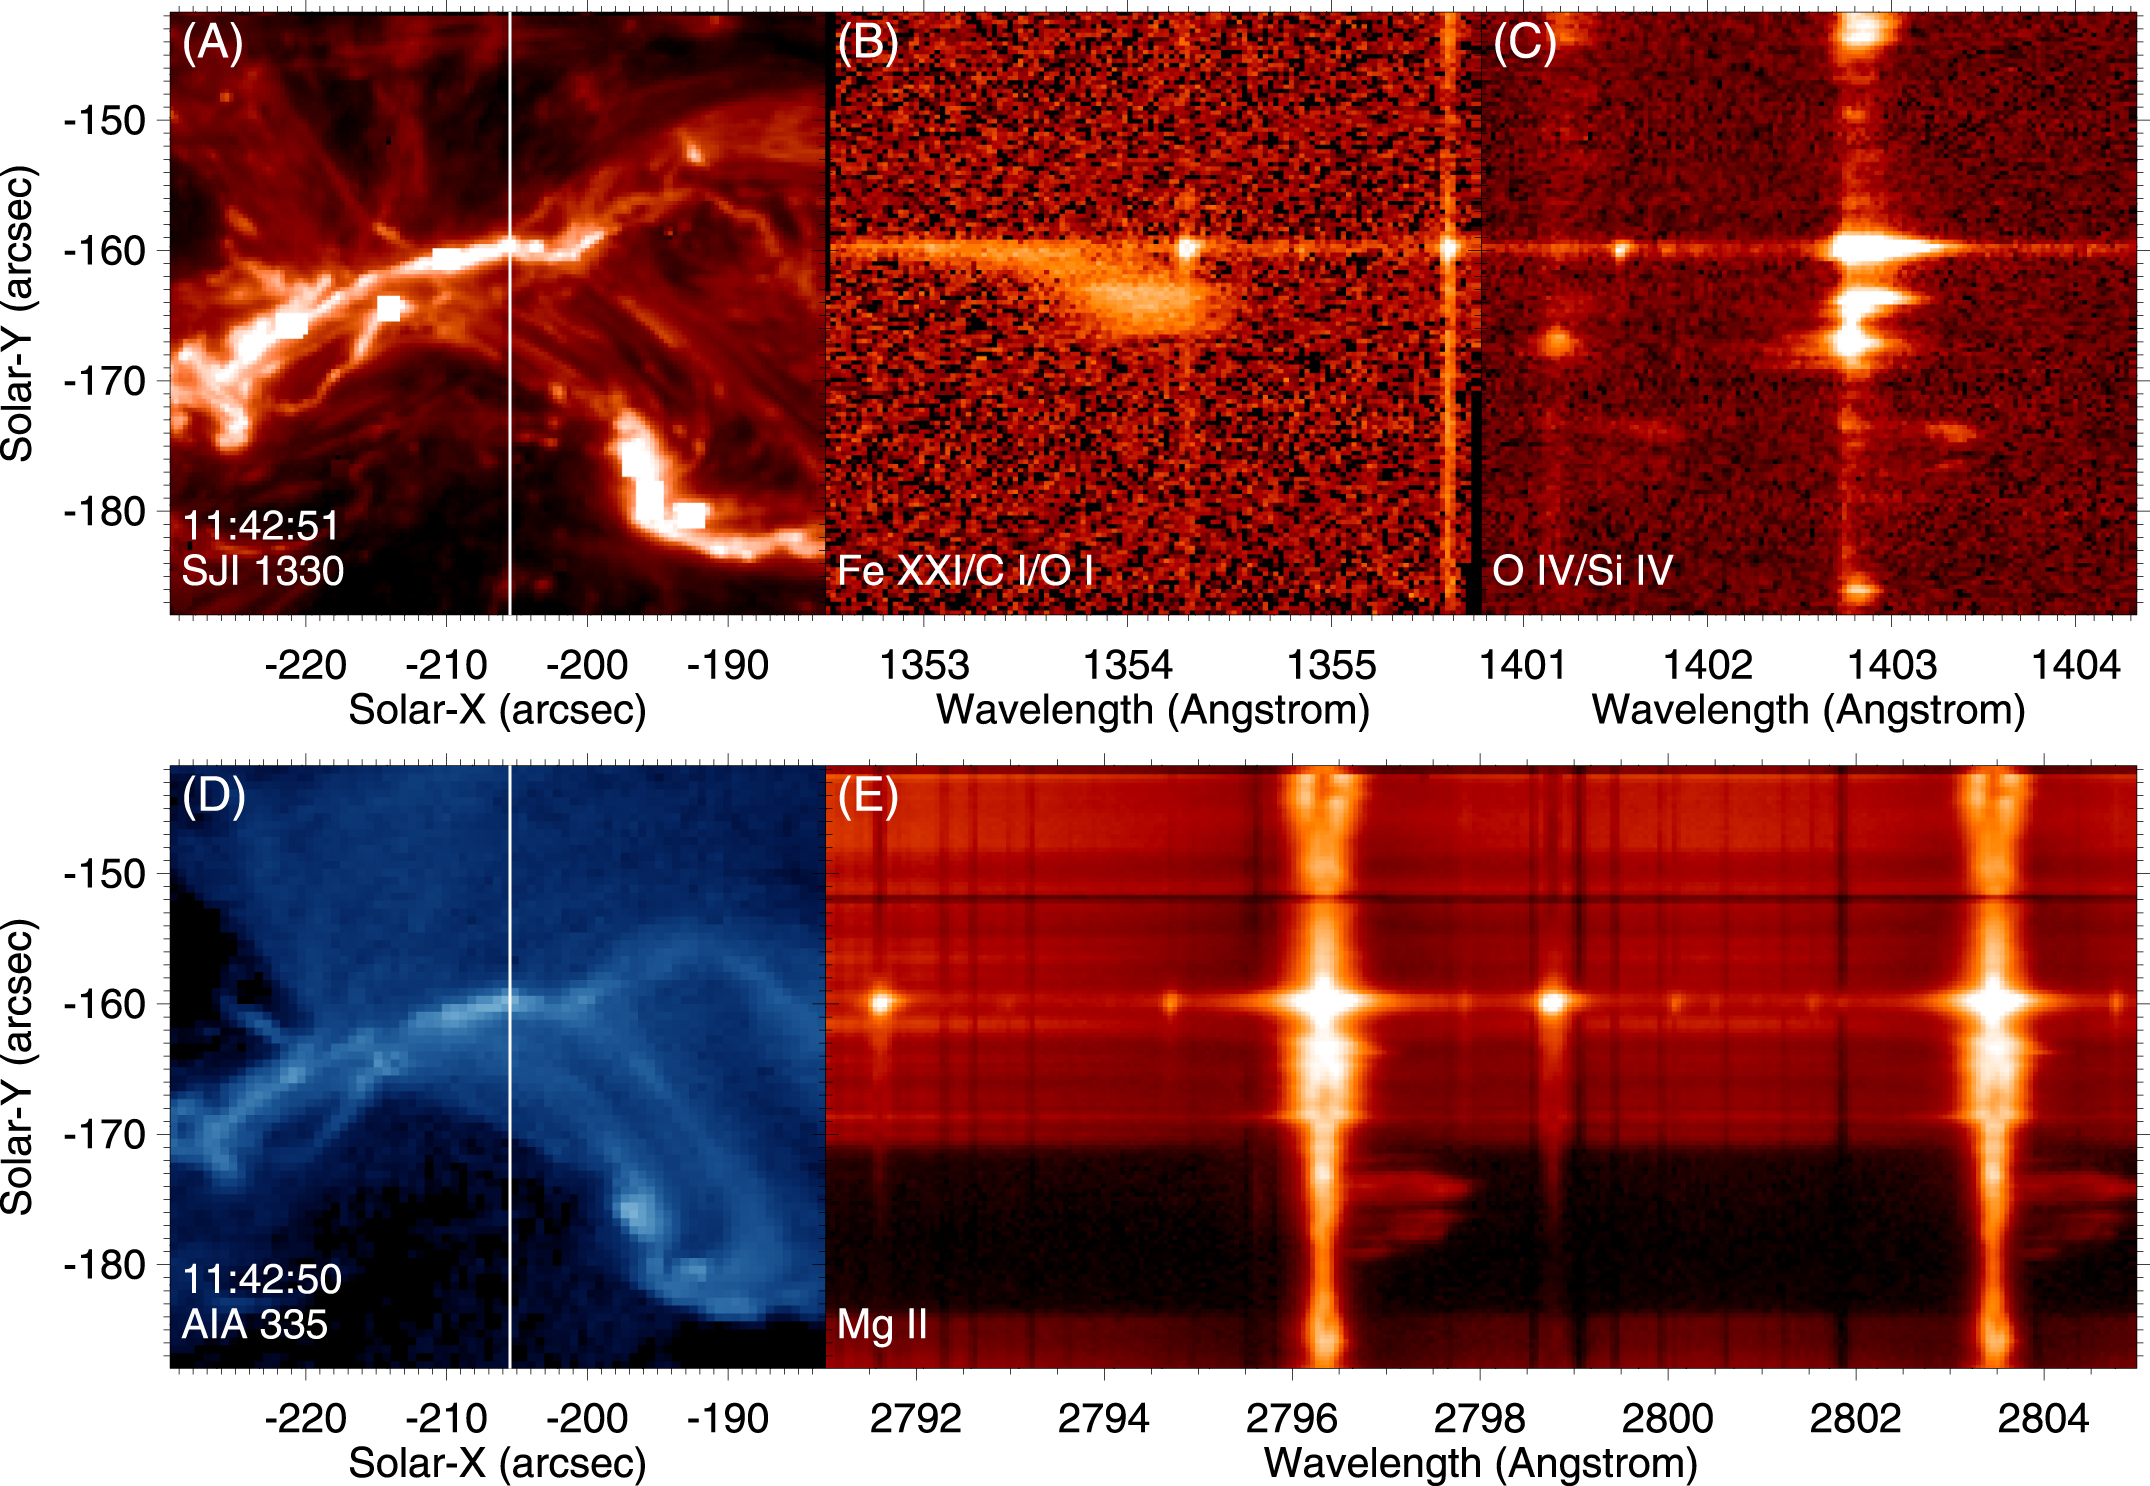
\includegraphics[width=0.7\linewidth]{figs/fig3}
	\caption{IRIS卫星对一个M1.6级耀斑带上谱线的观测,可以看到Si \textsc{iv},Mg \textsc{ii}等一系列谱线在耀斑带上都出现了红翼不对称性,而另一条高温谱线Fe XXI呈现出较大的蓝移。来源:\textcite{Tian2018}}
	\label{fig:3}
\end{figure}
另外近年来日冕中的三维磁重联过程也在极紫外(\textit{EUV})等一系列波段被观测到,这些耀斑不但具有复杂的日冕磁场拓扑结构,还表现出特殊的耀斑带形状,如环状耀斑带\parencite{Wang2012,Sun2013},J形耀斑带\parencite{Chandra2009}和X形耀斑带\parencite{Liu2016}等。这些特殊的耀斑带形状可以被一些三维的磁重联理论解释\parencite{Janvier2013,Janvier2014}。由于本文主要关注低层大气对入射非热电子束的动力学和热力学响应,因此对日冕中的三维磁重联过程及拓扑结构变化不再加以赘述。

对于这些低层大气的加热情况以及辐射转移的模拟也在近年来不断发展。以RADYN\parencite{Carlsson1992,Carlsson1997,Allred2005,Allred2015}为代表的一批辐射流体力学(\textit{radiative hydrodynamics, RHD})代码对我们认识耀斑加热时丰富的色球动力学过程提供了很大的帮助。通过计算色球中非局部热动平衡(\textit{nonlocal thermodynamics equilibrium, NLTE})条件下的辐射转移过程,我们得以了解色球中光学厚的一系列谱线的形成情况。关于这方面的研究成果,我会在\ref{sec:1.3}节中加以详细介绍。

\subsection{Ellerman炸弹}
Ellerman炸弹是太阳低层大气的爆发活动,最早在1917年被Ellerman在H$\alpha$线翼窄带滤光器的成像中观测到\parencite{Ellerman1917},表现为H$\alpha$线翼的增强\parencite{Georgoulis2002,Yang2003,Fang2006,Pariat2007,Nelson2013,Nelson2015,Vissers2015}。与之相反的,在H$\alpha$线心处一般观测不到增强。一般认为它们是太阳低层大气温度极小区(\textit{temperature minimum region, TMR})中的磁重联过程加热的结果\parencite{Reid2015,Rouppe2016,Ni2016}。其他形成于低色球的谱线,如Mg \textsc{ii}, Ca \textsc{ii}三重线也会在线翼出现增强,这些都被认为是低层大气加热的证据\parencite{Hong2017a,Nelson2017,Chen2017a},见图\ref{fig:4}。目前已有的一维辐射流体力学模拟和三维辐射磁流体力学(\textit{radiative magneto-hydrodynamics, RMHD})模拟,已经再现了Ellerman炸弹的部分光谱特征,如H$\alpha$的线翼增强等。\parencite{Hong2017a,Reid2017,Hansteen2017,Danilovic2017,Hansteen2019}。

\begin{figure}
	\centering
	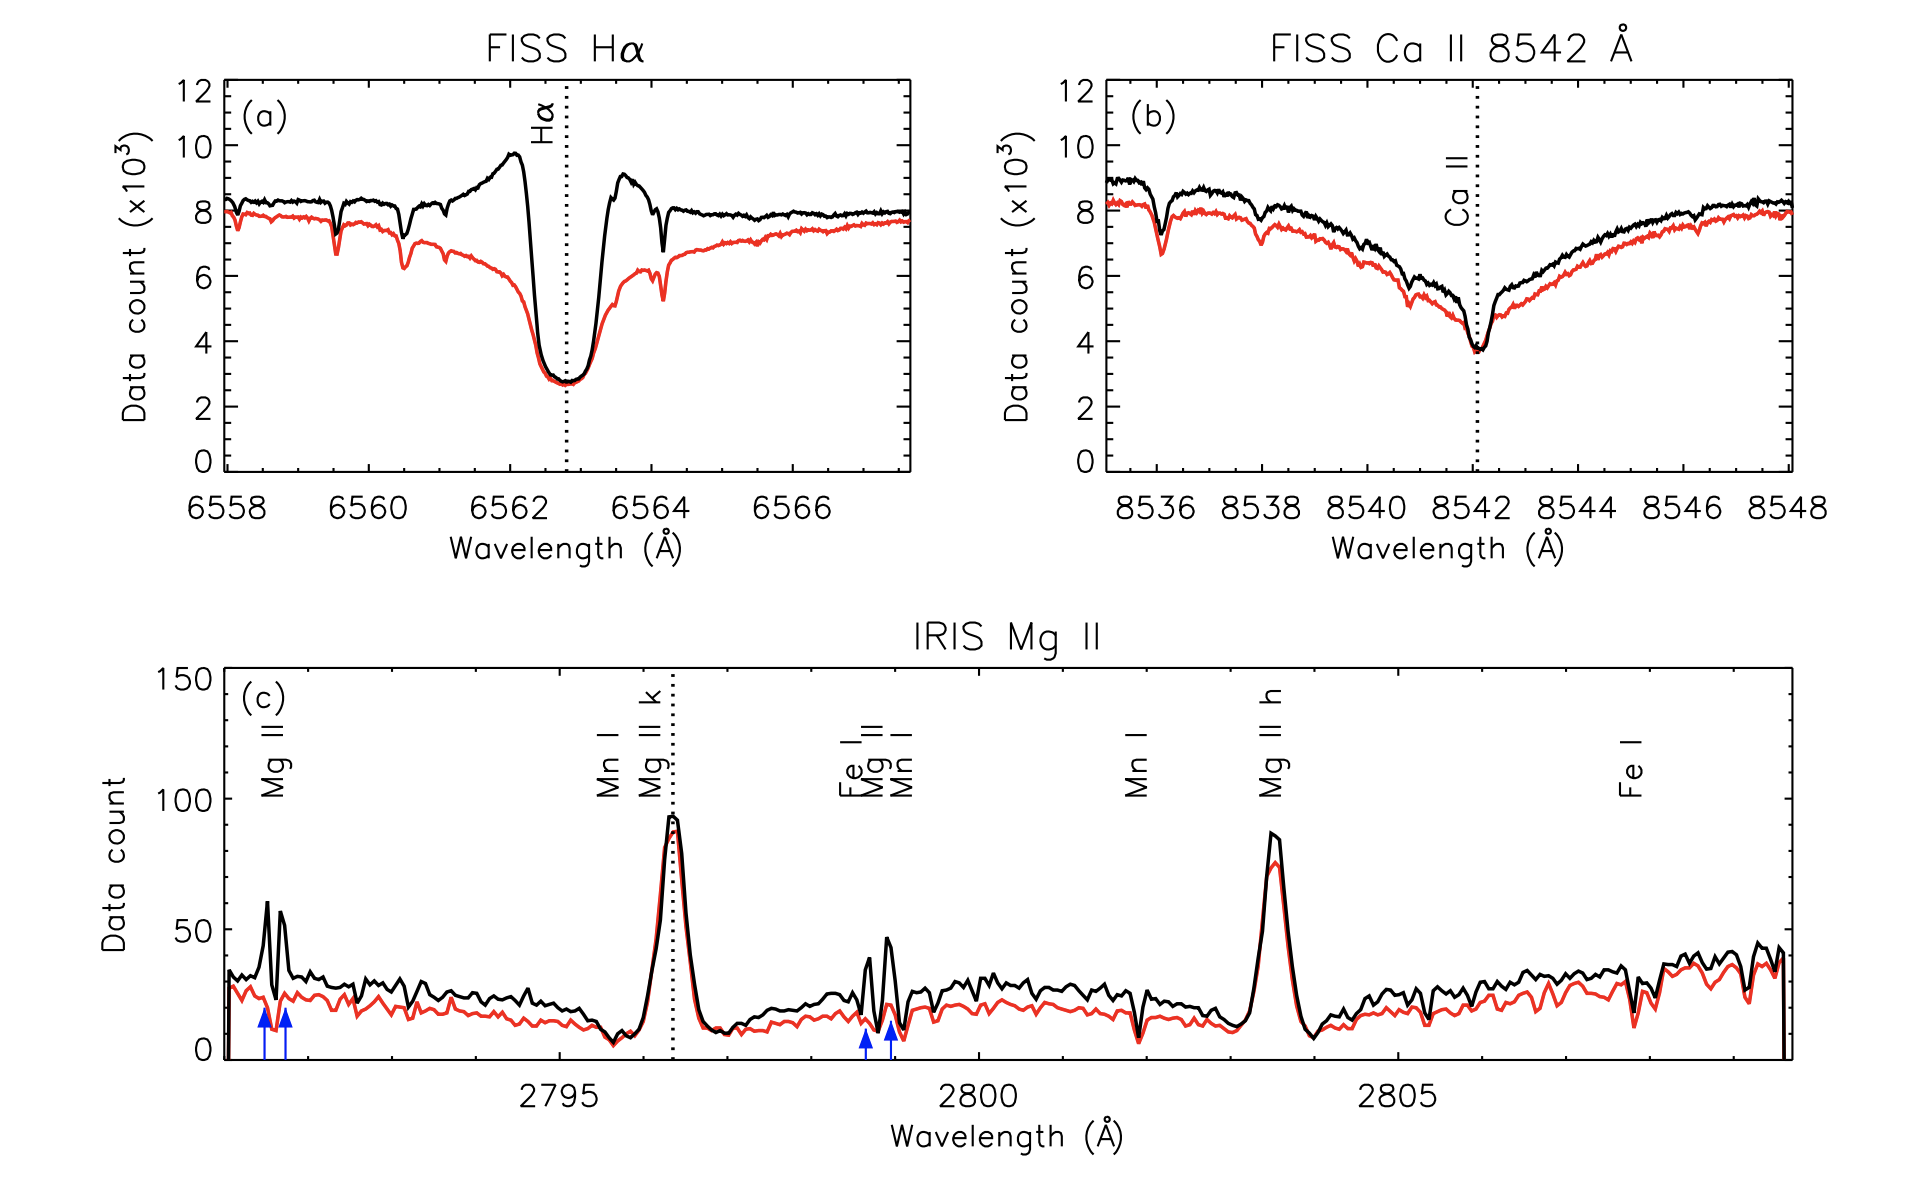
\includegraphics[width=0.8\linewidth]{figs/fig4}
	\caption{快速太阳成像光谱仪(\textit{Fast Imaging Solar Spectrograph, FISS})与IRIS卫星对一个Ellerman炸弹光谱的联合观测得到的光谱数据,红色和黑色的实现分别来自同一位置爆发前后的谱线轮廓。来源:\textcite{Hong2017a}}
	\label{fig:4}
\end{figure}
\subsection{紫外爆发}
紫外爆发(\textit{UV burst})是近年来新被观测到的一种位于色球层的小规模爆发活动,最早被过渡区成像摄谱仪(\textit{Interface Region Imaging Spectrograph, IRIS}: \cites{DePontieu2014})卫星于2014年在1400 \mbox{\AA}波段成像观测到\parencite{Peter2014},在最初也被称为热爆发(\textit{hot explosion}, \cite{Peter2014})和IRIS炸弹(\textit{IRIS bomb}, \cite{Tian2016})。紫外爆发经常出现在IRIS卫星对活动区(\textit{active region, AR})的观测当中\parencite{Tian2016,Polito2016,Hou2016}。在光谱观测上,紫外爆发表现为Si \textsc{iv} 和 C \textsc{ii}谱线的剧烈增强和致宽,其等值宽度能够达到$50-200\ \mathrm{km}\ \mathrm{s}^{-1}$, 同时在致宽的Si \textsc{iv} 1394\mbox{\AA}线上还经常能够观测到一条Ni \textsc{ii}的吸收线\parencite{Peter2014,Chen2019a},见图\ref{fig:5}。一般认为紫外爆发的能量来源于Ellerman炸弹类似,都来自于低层大气中的磁重联过程\parencite{Peter2014,Tian2018b},见图\ref{fig:6}。
\begin{figure}
	\centering
	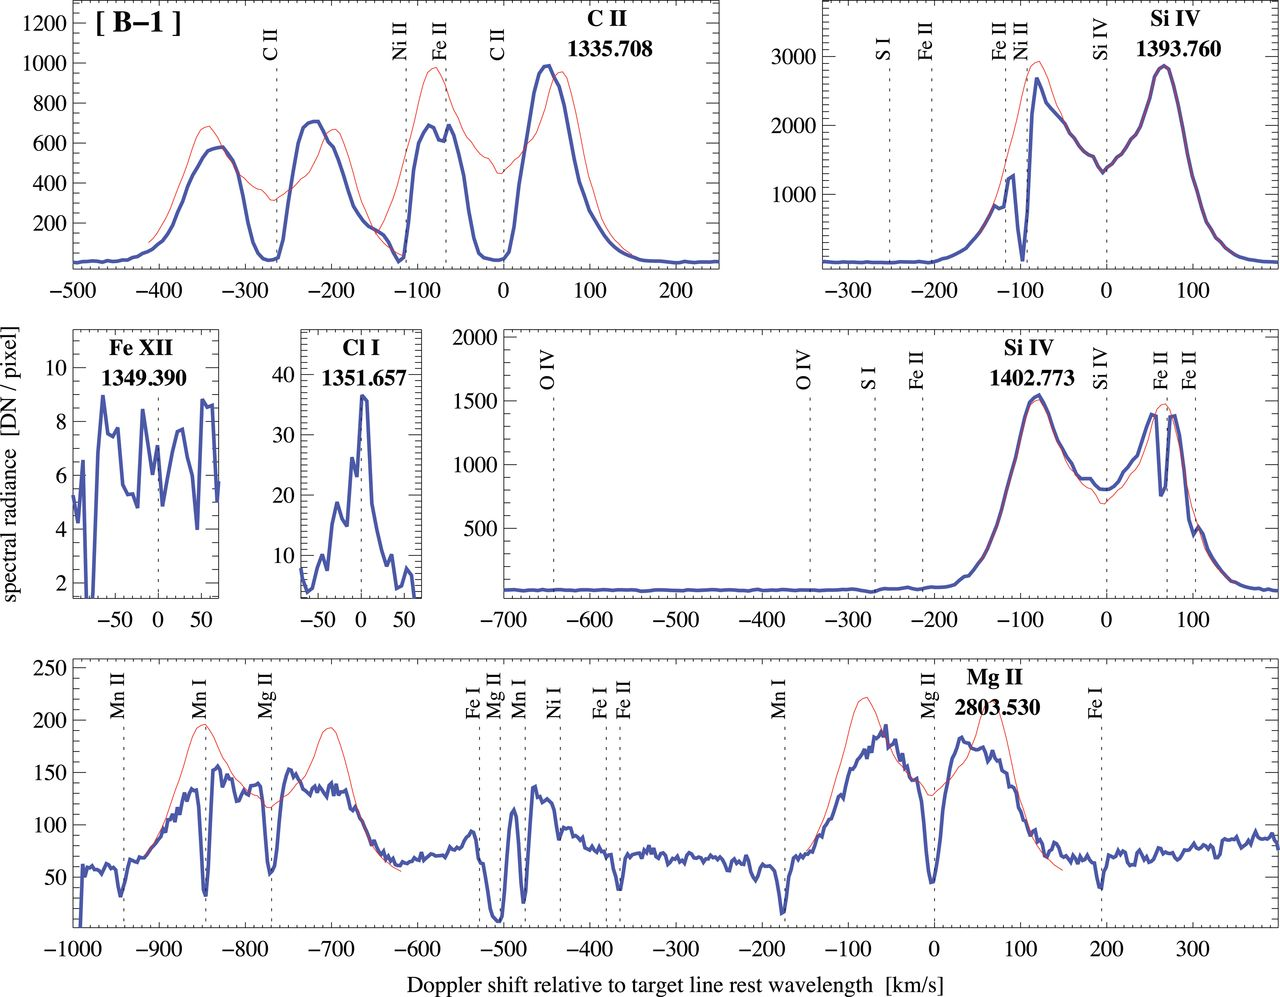
\includegraphics[width=0.7\linewidth]{figs/fig5}
	\caption{IRIS卫星观测到的紫外爆发的光谱。来源:\textcites{Peter2014}}
	\label{fig:5}
\end{figure}
\begin{figure}
	\centering
	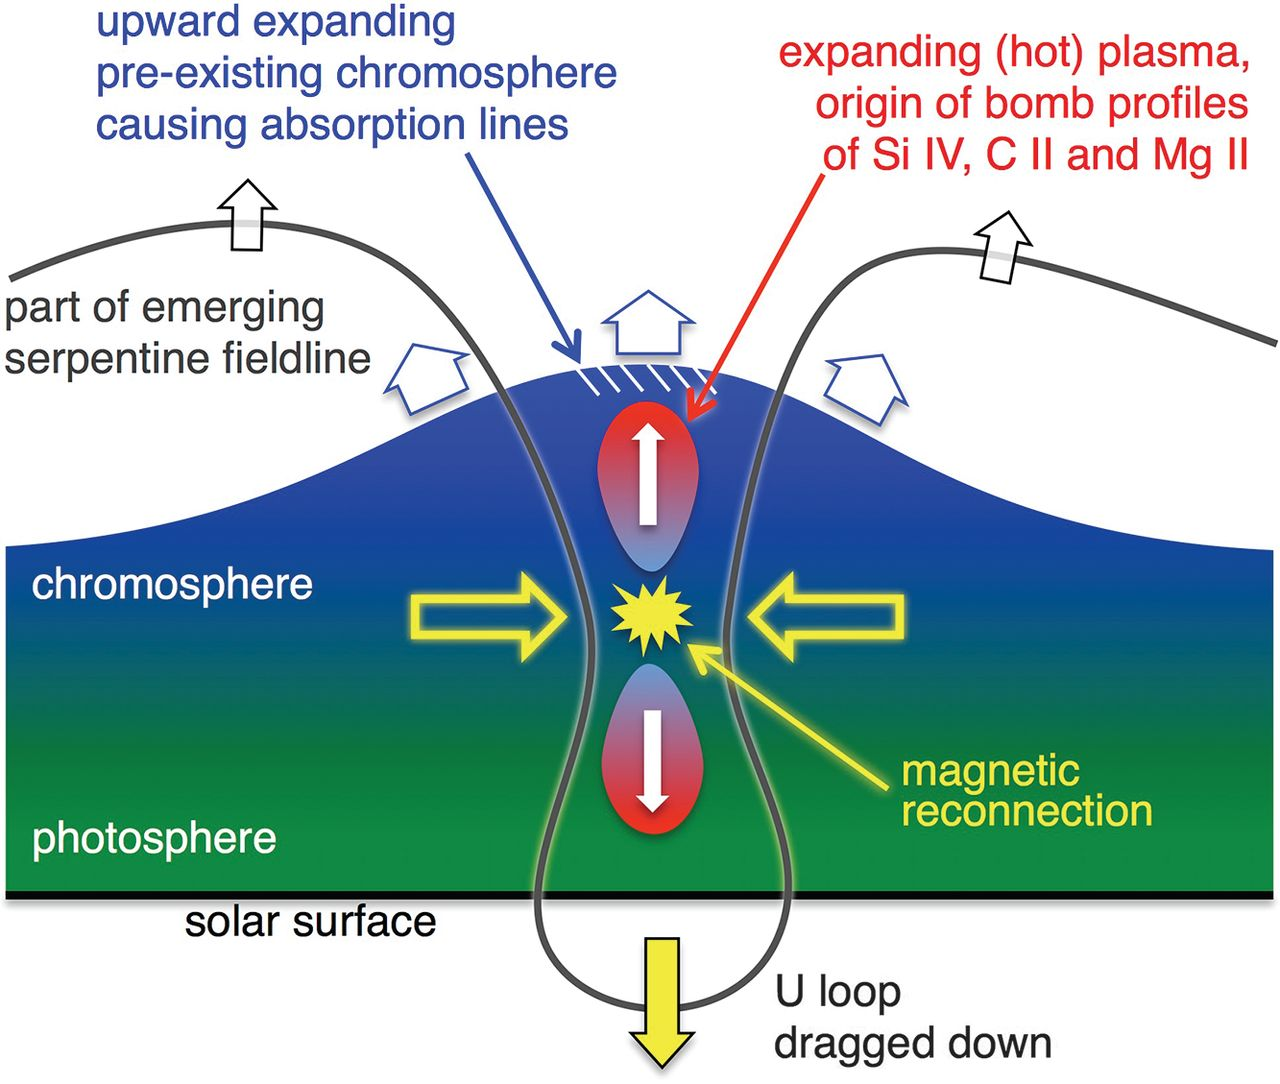
\includegraphics[width=0.7\linewidth]{figs/fig6}
	\caption{一个用于解释紫外爆发成因的卡通图。\textcite{Peter2014}认为色球层中的倒U型磁感线间的磁重联过程加热了局部色球大气,这些物质的向上蒸发导致了急剧增强和致宽的Si \textsc{iv}, C \textsc{ii}等线。在这些蒸发物质的上方存在的较冷的色球大气造成了Ni \textsc{ii}等覆盖在发射谱线上的吸收特征。来源:\textcites{Peter2014}}
	\label{fig:6}
\end{figure}

近年来的一些观测表明,紫外爆发和Ellerman炸弹存在着一定的关联性\parencite{Vissers2015,Tian2016},它们的形成机制也有一定的相似之处。\textcite{Fang2017}表明发生在低层大气的Ellerman炸弹并不足以加热附近的温度极小区到达$10^4$ K,进而电离足够的Si \textsc{iv}离子产生Si \textsc{iv}谱线增强。\textcite{Chen2019a}对Goode太阳望远镜观测到的161个Ellerman炸弹进行了统计分析,发现仅有约20个Ellerman炸弹能够在IRIS卫星观测中找到对应的紫外爆发,而且这些紫外爆发往往位于对应的火焰状Ellerman炸弹的上方。他们指出这些相关的Ellerman炸弹和紫外爆发可能形成发生在同一个电流片上的在不同高度的磁重联过程中(见图\ref{fig:7})。Hansteen等人近年来一直使用Bifrost三维辐射流体动力学代码对Ellerman炸弹和紫外爆发的光谱特征进行计算,也成功再现了Si \textsc{iv},H$\alpha$等一系列谱线轮廓特征。他们发现紫外爆发和Ellerman炸弹可以是在空间和时间上都不关联的两个爆发活动\parencite{Hansteen2017},但它们也可以同时形成在同一狭长电流片的两端\parencite{Hansteen2019}。
\begin{figure}
	\centering
	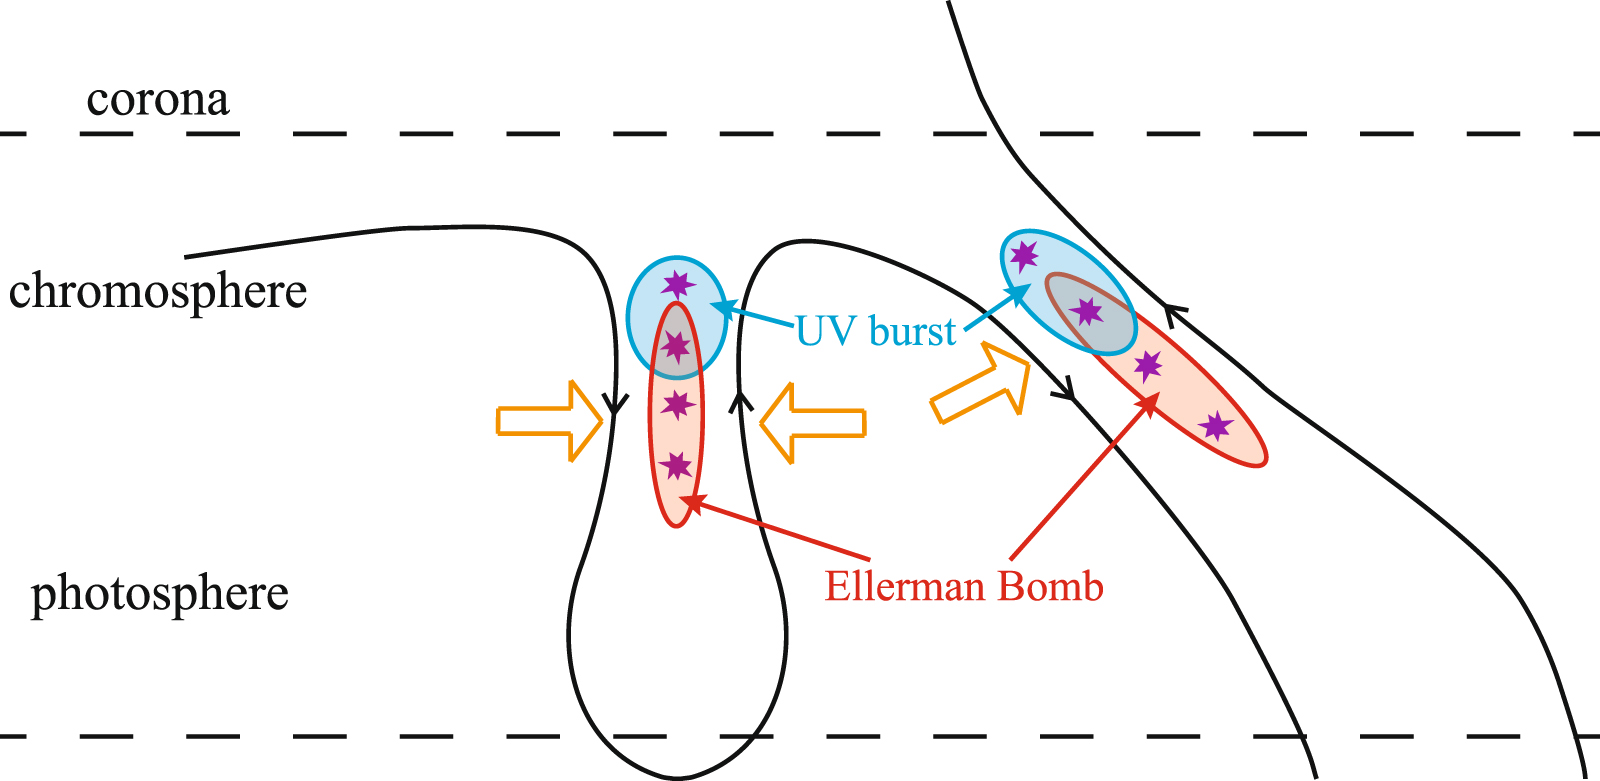
\includegraphics[width=0.7\linewidth]{figs/fig7}
	\caption{一个用以解释Ellerman炸弹与紫外爆发形成在同一电流片上的卡通图。来源:\textcites{Chen2019a}}
	\label{fig:7}
\end{figure}
\subsection{M矮星上的恒星耀斑}
近年来,随着地基和太空望远镜的发展,恒星耀斑也越来越多地被在测光(\textit{photometric})和分光(\textit{spectroscopic})观测中被探测到,并且展现出特殊的辐射特征。尤其是在一些M矮星上,如UV Ceti,YZ CMi和比邻星上都观测到了较强的白光耀斑,释放出比太阳耀斑高出一个量级以上的能量\parencite{Haisch1989}。统计研究表明光谱型介于dM3e-dM6e间的M矮星常常能观测到频繁的耀斑爆发\parencite{Lacy1976}。这些耀斑的光变曲线和太阳耀斑类似,都包含了一个快速增长的爆发相和一个持续几十分钟到几个小时的衰变相\parencite{Moffett1974,Moffett1976}。

在测光观测上,随着Kepler卫星\parencite{Borucki2010}的发射,大视场长周期的白光观测在M矮星和一些类太阳的G型星上都观测到了大量的耀斑活动和恒星黑子\parencite{Shibayama2013,Hawley2014,Davenport2014,Lurie2015,Yang2017}。这些白光耀斑往往在U波段(3200\mbox{\AA}-4000\mbox{\AA})光度学观测上显示出比较大($\Delta U\sim5\ \mathrm{mag}$)的变化\parencite{Haisch1989}。同时宽波段(U,B,V和R)的测光观测指出耀斑在白光波段的增强可能与一个$T\sim 9000-10000$ K的黑体谱相似\parencite{Hawley1991,Hawley1992}。在2018年发射的凌星系外行星巡天望远镜(\textit{Transiting Exoplanet Survey Satellite, TESS}: \cites{Ricker2014})发射开始观测后的两个月内,利用其高分辨率(2分钟)的观测数据,就发现了632颗发生过耀斑活动的M矮星\parencite{Gunther2019}。这些数据充分说明了频繁的恒星活动对系外行星宜居性的重要影响。

相比于长周期和大视场的测光巡天,恒星耀斑的分光观测往往较为困难,因为它们的出现往往是不可预测的。一般来说耀斑事件都伴随着连续谱增强及H$\alpha$等Balmer线系,Ca \textsc{ii}, Mg \textsc{ii},He \textsc{i}, K \textsc{i}等一系列色球谱线的增强和致宽\parencite{Eason1992}。\textcite{Hawley2007}利用Hubble太空望远镜上的空间望远镜成像光谱仪(\textit{Space Telescope Imaging Spectrograph, HST/STIS})观测了YZ CMi上的一个恒星耀斑的NUV光谱中的Mg \textsc{ii}和Fe \textsc{ii}线。其中Mg \textsc{ii}线展现出了剧烈的增宽,其半高全宽(\textit{full width at half maximum, FWHM})一度达到了250 $\mathrm{km}\  \mathrm{s}^{-1}$。YZ CMi上的白光耀斑和太阳上的\textsc{i}型白光耀斑类似,在Balmer系限3646\mbox{\AA}附近出现蓝段连续谱辐射的突然增强,被称为Balmer跳跃\parencite{Kowalski2010}。Balmer跳跃一般认为来自于氢原子与自由电子的复合(\textit{recombination})过程,因此着预示着白光连续谱不仅具有一个黑体谱的成分,还有来自于氢原子复合连续谱的分量\parencite{Kowalski2012}。\textcites{Kowalski2013}对20个M矮星上的恒星耀斑进行了光谱和光度的联合观测,他们发现可见光谱在$4000-4800$\mbox{\AA}间的部分可以被一个温度较高的9000-14000 K的黑体谱所拟合,而$\lambda>4900$ \mbox{\AA}的光谱则可以被一个温度较低$\sim6000$ K左右的黑体谱拟合。在这些耀斑中的Balmer线系谱线的线翼都出现了吸收的现象,这一特征被认为是低层大气被加热的证据。他们最近对两个发生在一个dM4e型矮星上的耀斑进行了联合观测,并首次利用Hubble太空望远镜上的宇宙起源光谱仪(\textit{Cosmic Origin Camera, HST/COS})获得了耀斑在大部分NUV波段的光谱数据,包含了增强的Balmer连续谱和大量的Fe \textsc{ii}和Mg \textsc{ii}线\parencite{Kowalski2019}。根据这些多波段的光谱观测,他们发现$T = 9000$ K的黑体谱并不能很好的拟合这两个耀斑事件的连续谱,尤其是在NUV波段。\textcite{Froning2019}对另一颗M矮星GJ 674的观测更揭示了耀斑过程中大量的FUV发射线,如Si \textsc{iii},O \textsc{iii},C \textsc{iii},Fe \textsc{xxi}等。

对这些M矮星耀斑的辐射流体力学模拟也同太阳耀斑模拟一样在近年来不断发展,不过目前主要还停留在再现恒星耀斑中的可见光连续谱和Balmer系谱线轮廓上。早期利用RADYN进行的模拟揭示了一系列增强的谱线,如H$\alpha$,H$\beta$, Ca \textsc{ii} H和K,He \textsc{ii} 304\mbox{\AA}等,但未能再现辐射温度较高的黑体连续谱\parencite{Allred2006},且不能再现剧烈致宽的Mg \textsc{ii}线\parencite{Hawley2007}。Kowalski等人在后来发现,要想再现这样剧烈增强的连续谱,需要在模拟中引入较高能量的非热电子束($1\times10^{13}\ \mathrm{erg}\ \mathrm{s}^{-1}$,以下简称F13,比普通太阳耀斑的模拟高至少两个量级,参见\cite{Kowalski2015})。同时使用一些更精确的Balmer线系的Stark致宽效应的计算方法,对整个耀斑的在3500 \mbox{\AA}-5000 \mbox{\AA}的连续光谱和Balmer发射线取得了非常好的拟合效果\parencite{Kowalski2015,Kowalski2016,Kowalski2017b}。和太阳耀斑类似,在M矮星的高非热电子能流模拟中也得到了色球凝聚的结果。这些模拟结果得到的大气参量可以帮助我们估计可见光和NUV波段的光学深度,Balmer跳跃比和色球凝聚处的电子密度等\parencite{Kowalski2018a}。
\section{辐射转移与谱线形成理论简介}
辐射转移(\textit{radiative transfer, RT})是恒星大气中重要的物理过程,最早由Schuster在1905年归纳给出辐射转移方程\parencite{Schuster1905}。它既是恒星大气中能量传输(加热、冷却)的重要手段,又是天体物理中绝大多数观测量即电磁波谱的形成机制。正确地理解辐射转移过程,不仅有助于我们处理流体力学方程组中能量方程的辐射项,又能够直接合成光谱和我们观测到的电磁波谱中的各种特征(连续谱、谱线等)进行比较,直接检验我们对太阳爆发时低层大气认识的正确性。在这一部分,我将介绍与辐射有关的物理量与辐射转移方程。谱线轮廓形成和致宽的机制和存在磁场情况下对光的偏振参数影响。限于篇幅,研究内容和个人能力限制,对辐射转移过程的介绍是比较简单的:我只介绍一维平面平行层大气的辐射转移过程,且只涉及静态大气不含时的辐射转移方程(事实上在模拟中存在速度场,显然不能以静态大气处理)。另外,我们讨论的主要是宏观上的辐射转移,即用一些宏观测量量来描述辐射场,而非光子数密度这样的微观量,尽管光子的概念在谱线形成的过程中仍然非常重要。本节的主要内容及公式都来自于Hubney和Mihalas所著的《Theory of Stellar Atmospheres》一书\parencite{Mihalas2014}。
\subsection{辐射转移方程}\label{subsec:1.2.1}
在介绍辐射转移方程之前,有必要介绍一些描述辐射场的物理量和重要概念:

\noindent
\textbf{辐射强度(Intensity)}\ \ 我们通过衡量单位时间$\delta t$通过单位面元$\delta\boldsymbol{A} $以某个方向$\boldsymbol{n}$通过单位立体角$\delta \Omega$在频率区间$(\nu,\nu+\delta\nu)$的辐射能量$\delta E$来衡量辐射强度的大小,即
\begin{equation}
	I(\boldsymbol{x},t,\boldsymbol{n},\nu ) = \frac{\delta E}{\delta t  \delta \Omega \delta \nu \delta\boldsymbol{A} \  \boldsymbol{n}}
\end{equation}
其在SI单位制下的单位为$\mathrm{W}\ \mathrm{m}^{-2}\ \mathrm{Hz}^{-1}\ \mathrm{sr}^{-1}$,在CGS单位制下单位为$\mathrm{erg}\ \mathrm{s}^{-1}\ \mathrm{cm}^{-2}\ \mathrm{Hz}^{-1}\ \mathrm{sr}^{-1}$。

\noindent
\textbf{辐射流量(Flux)}\ \ 辐射流量$\boldsymbol{F}_{\nu}$被定义为使得$\boldsymbol{F}_{\nu}\ \md \boldsymbol{A}$给出单位时间内通过面元的在频率间隔$\md \nu$内的能流,因此我们要对单位角进行积分
\begin{equation}
	\boldsymbol{F}_{\nu} = \oint_{4\pi} I_{\nu}(\boldsymbol{n} )\boldsymbol{n}\md \Omega
\end{equation}
在恒星当中,由于我们往往只对向观测者方向传播的能量感兴趣,因此观测到的辐射流量一般只积$\theta\in (0,\pi/2)$之间。

\noindent
\textbf{局部热动平衡(Local Thermodynamic Equilibrium, LTE)}\ \ 在恒星大气物理的研究当中,局部热动平衡是永远无法回避的一个概念。我们大多数关于辐射场和原子电离激发的知识是适用于平衡态的,如Boltzmann分布和Saha方程等。但是显然恒星大气存在温度梯度,并不是一个完全的热平衡态。为了做出一个合适的近似,一个很自然的想法是,如果局部的温度梯度和密度梯度是\emph{充分小}的,且粒子密度\emph{充分大}以保证充分的碰撞,那么我们就可以用一些“局部”的大气动力学、热力学参数来描述一个“局部”范围内的大气,并认为这个范围内的大气处于一个平衡态当中,这就是局部热动平衡的概念。这个“充分小”可以理解为温度和密度的标高应该远大于粒子的自由程\parencite{Mihalas2014}。但是我们也应该注意到光子很可能拥有比普通粒子大的多的自由程,因为整个外辐射场是通过一系列辐射与吸收机制(对应粒子的电离、受激、复合和退激发过程)与粒子耦合在一起来趋向平衡态的。因此检验这个近似是否在恒星大气中严格成立事实上在不依靠数值模拟的情况下是比较困难的。

总的来说,局部热动平衡在恒星大气的光球是一个比较好的近似,但是在色球很可能不是,这也是为什么我们需要非局部热动平衡(\textit{non-LTE, NLTE})的概念\parencite{Mihalas2014}。理论上来说,任何对于LTE的偏离都应该算作NLTE的范畴内,但是在具体代码计算中,比较常用的方法是假设粒子的速度分布仍然满足平衡态下的Maxwellian分布,但原子能级粒子数分布则可以偏离Boltzmann分布和Saha方程给出的限制\parencites{Kubat2014}。由于此时的能级粒子数分布应该由动理学平衡(\textit{kinetic equilibrium})方程给出,因此此时也被称为统计平衡(\textit{statistical equilibrium})或动理学平衡\parencites{Mihalas2014}。

\noindent
\textbf{吸收(Absorption),发射(Emission)与散射(Scattering)}\ \ 当一个光子和粒子相互作用而消失的时候,我们一般说它被\emph{吸收}了。而如果粒子失去一部分能量而释放出一个光子,我们就称之为\emph{发射}。如果这个光子的能量一部分通过碰撞激发与电离进入交换给了其他粒子,那么我们一般称这是\emph{热(真)吸收}(\textit{thermal absorption})。反之,如果它激发了一个原子从某个能级$l$跃迁到$u$,而这个原子又很快退激发回到$l$发出一个频率大致相等的光子,那么这个过程应该被称作\emph{散射}(\textit{scattering}),因为光子的能量并没有介入到粒子的内能中去。这两个过程的重要区别是热吸收的再辐射应该是遵循处于热动平衡下的辐射场性质的,而散射过程的再辐射却不遵循这些性质。

然而,我们应该指出,在真实情况下,由于原子有着复杂的能级和电离结构,一个光子被吸收然后再被释放的中间过程是非常复杂的,很难直接用吸收或者散射的概念来严格描述。在某些情况下,如果只考虑光子被吸收的过程而不考虑它是如何再发射的,我们会宽泛地把散射过程也归纳到吸收中来考虑。

对于造成光子被吸收和发射有着各种各样的物理过程,我们不再这里对它们的物理形式做过多的数学描述,只是走马观花式地罗列恒星大气中可能造成吸收的物理过程。可以吸收或辐射宽波段光子的过程一般包括\parencite{Wang1993}:
\begin{itemize}
	\item 光致电离与复合(\textit{photoionization, recombination})
	\item 自由-自由跃迁/轫制辐射 (\textit{free-free transition/bremsstrahlung})
	\item 分子离解、电离和分子带吸收
	\item Thompson散射与Rayleigh散射
	\item 尘埃的散射和吸收
\end{itemize}
而与之相对应的就是谱线内部的跃迁(\textit{bound-bound transition})。具体而言,包含自发辐射(\textit{spontaneous emission}),受激辐射(\textit{stimulated emission})与光致激发(\textit{photoexcitation})。


现在我们可以开始讨论一维平面平行层大气辐射的传播过程应该用什么样的方程和参量来描述了,为了定量描述辐射在局地的吸收和发射过程,我们可以定义两个参量,\emph{不透明度}$\chi_\nu$(\textit{opacity})与发射系数$\eta_\nu$(\textit{emissivity})。前者描述了单位的辐射强度通过单位距离后的改变量。在考虑散射的情况下而后者描述了辐射通过单位距离物质之后的增强量,考虑这两个参数同时对辐射强度的影响,我们有
\begin{equation}
	\md I_{\mu\nu} = \left(\eta_{\nu} - \chi_{\nu}I_{\mu\nu}\right) \mu \md z
\end{equation}
其中$\mu=\cos\theta$表示辐射出射方向与平面大气法线方向的夹角的余弦,$z$表示大气高度,$I_{\mu \nu}$表示以某一方向出射的辐射强度。注意我们为了尽可能简单的提取辐射转移的物理特征,在写下这个方程的时候已经做了非常多的假设。其中最重要的假设是吸收和发射都是\emph{各向同性的}。事实上这是一个并不好的假设,因为显然一系列散射过程,如Thompson散射的再发射系数就是非各向同性的。下面我们继续改写这个方程,两边同除$\chi_\nu \mu \md z$,得到
\begin{equation}
	\mu \frac{\md I_{\mu \nu}}{\chi_\nu\md z} = \frac{\eta_\nu}{\chi_\nu} - I_{\mu \nu}
\end{equation}
下面我们定义另外两个重要的参量,光学深度(\textit{optical depth}) $\md \tau_\nu \equiv \chi_\nu \md z$与源函数(\textit{source function}) $S_\nu \equiv \eta_\nu / \chi_\nu$。前者为我们提供了判断一条谱线辐射转移中吸收是否重要的判据。一般来说$\tau = \int \chi_\nu \md z > 1$时,我们称之为光学厚(\textit{optically thick}),说明谱线形成中的吸收是不可忽略的。反之则称之为光学薄(\textit{optically thin}),说明吸收过程并不重要。此时我们观测到的谱线内的辐射可以直接理解为视线方向上所有发射的积分。而后者从形式上来看表示的是发射和吸收之比,但其还有一个重要的物理意义,即\emph{单位光深所能发射出的光子数}\parencites{Mihalas2014}。所以现在方程写作
\begin{equation}
	\mu \frac{\md I_{\mu \nu}}{\md \tau} = S_{\nu} - I_{\mu \nu}
\end{equation}
这一方程对出射辐射的形式解为
\begin{equation}
	I_{\mu \nu} = \frac{1}{\mu} \int^\infty_{\tau_\nu} S_{\nu} e^{-(t_\nu - \tau_\nu)} \md t_\nu \label{eq:1.6}
\end{equation}
由于$S_{\nu}$也是光学深度$\tau_\nu$的函数,所以这仍然是一个形式解。但从这个解的形式可以看出,与一般的流体力学方程不同,想要计算出射的辐射强度,这个积分将涉及整个太阳大气,因此求解这样的方程是非常消耗计算时间的。最后我们讨论一下同时考虑热吸收和散射时和LTE假设下的源函数的形式。在LTE下,热吸收和热发射应该遵循热平衡下的辐射场性质(即Kirchhoff热辐射定律) $\eta_{\nu,\mathrm{thermal}}/\chi_{\nu,\mathrm{thermal}} = B_{\nu}$,其中$B_\nu$为Planck函数。我们可以把$\eta_\nu$和$\chi_\nu$分解写成热吸收和散射两个部分
\begin{align}
	\chi_\nu &= \kappa_\nu + \sigma_\nu \\
	\eta_\nu &= \kappa_\nu B_\nu + \sigma_\nu J_\nu
\end{align}
其中$\kappa_\nu$和$\sigma_\nu$分别代表热吸收和散射的吸收系数,$J_\nu$代表立体角平均后的辐射强度。因此在这样的近似下源函数的形式可以写成\parencites{Mihalas2014}
\begin{align}
	S_\nu &= \frac{\kappa_\nu B_\nu + \sigma_\nu J_\nu}{\kappa_\nu + \sigma_\nu} \nonumber \\
	& = \epsilon_\nu B_\nu + (1-\epsilon_\nu )J_\nu
\end{align}
\subsection{谱线形成分析}\label{sec:1.2.2}
太阳上的原子谱线最早被Fraunhofer在1814年观测到,这也是最早被观测到的原子能级跃迁产生的吸收线。那么如何判断一条谱线是在太阳大气的何种高度,进一步的,何种大气参数下形成的呢?一个简单的想法是根据太阳大气的温度分布,依照原子电离态可能在何种温度区间下存在的信息,进而粗略地推断谱线的形成高度。这显然是一个非常粗略的方法,而且对于吸收效应比较重要的谱线,即光学厚的谱线,我们观测到的光子往往是经过了多次的散射过程才形成的。在这样的情况下,我们观测到的谱线轮廓中的光子往往仅形成在整个电离态原子可能存在高度的较高处。对于这些谱线,基于\ref{subsec:1.2.1}节中讨论的辐射转移方程,我们可以把光学深度$\tau_\nu = 1$的高度当作是谱线形成的特征高度,因为此处发射的光子大约有$1 - e^{-1}\approx63\%$可以被我们观测到。下面为了更好的确定整个谱线的形成区间,并对谱线形成高度的大气参数进行一个定量分析,我们介绍一种基于贡献函数$C_{I}$\parencite{Magain1986,Carlsson1997,Kowalski2015}的方法。

首先我们把辐射转移方程形式解式\eqref{eq:1.6}中的被积函数定义为贡献函数$C_I(\mu,z) \equiv \md I_{\mu \nu}/\md z = \chi_\nu S_\nu e^{-(t_\nu-\tau_\nu)}$,因此所有的出射辐射强度可以视作整个贡献函数对大气高度的积分。自然地,贡献函数大的地方就应该是谱线真正形成的地方。为了更加定量的描述这一点,我们可以定义一个积累(\textit{cumulative})贡献函数$C'_I(\mu,z)$\parencite{Kowalski2016b}。
\begin{equation}
    C'_I(z,\mu) = 1- \frac{\int^{z'=z_{\mathrm{max}}}_{z' = z} C_I(z',\mu)\ \mathrm{d}z'}{\int^{z'=z_{\mathrm{max}}}_{z' = z_{\mathrm{min}}} C_I(z',\nu)\ \mathrm{d}z'}
\end{equation}
这是一个归一化的函数,进一步的,我们可以定义$C'_I \in (0.05,0.95)$作为谱线的形成区间。另外我们可以利用贡献函数$C_I$作为一个权重函数,对模拟中的大气参数在高度上做加权平均,作为谱线形成区间内的典型大气参数,即
\begin{equation}
    <X> = \frac{\int^{z\left(C'_I=0.95\right)}_{z\left(C'_I=0.05\right)}C_I(z',\mu)X\ \mathrm{d}z'}{\int^{z\left(C'_I=0.95\right)}_{z\left(C'_I=0.05\right)}C_I(z',\mu)\ \mathrm{d}z'}
\end{equation}
其中$X$可以是温度、电子密度和速度等一系列参量。
\subsection{谱线的致宽}\label{sec:1.2.3}
尽管我们知道原子跃迁的能级差应该是确定的,但是观测到的谱线永远不会是一个$\delta$函数。除了测量造成的致宽之外,有许多物理效应可以造成谱线在辐射转移过程中的致宽。在这一小节,我会对谱线的致宽机制和谱线形状做出一个简单的总结。我将回避复杂的数学推导而尽量给出一个直观的物理图像和最后的数学结论。
\newline
\newline
\noindent
\textbf{自然致宽}\ \ 谱线的自然致宽来自于谱线跃迁的量子力学效应。简单地来说,在非相对论量子力学中,利用含时微扰论我们可以得到在一个受微扰的系统中,如果某个微小的能量变化$\Delta E$有较大可能在前后两次间隔时间为$\Delta t$的测量中出现,两者应该大致满足关系$\Delta E \Delta t \sim \hbar$。换句话来说,由于束缚电子处于一个能级的时间是有限的,故其的能量也并非完全确定的,而是存在一定的几率分布。通过Fourier变换,我们可以得到某条谱线的自然致宽在频率空间应该满足一个Lorentz分布:
\begin{equation}
	\phi_{ij}(\omega) = \frac{\Gamma_{ij}/2}{(\omega - \omega_{ij})^2 + (\Gamma_{ij}/2)^2}
\end{equation}
其中$\Gamma_{ij}$是由上下能级的自发跃迁和受激跃迁共同决定的。在具体分布中,它就是Lorentz形谱线的半高全宽(\textit{full width at half maximum, FWHM})。

\noindent
\textbf{微观Doppler致宽}\ \ 由于恒星大气中的原子一直处在热运动和微湍动(\textit{microturbulence})当中,这些运动的自由程远小于光子自由程,因此被称为是微观的。由于Doppler效应,这些原子发出的光子的频率发生了移动。因此在观察者看来,这些谱线被致宽了。一般来说我们认为这些原子的热运动和微湍动的速度分布都应该满足Maxwellian分布,因此最后得到的谱线满足Gaussian (Maxwellian)分布。
\begin{equation}
	\phi_{ij}(\omega) \propto e^{-(\omega^2-\omega_{ij})^2/\Delta \omega^2}
\end{equation}
其中$\Delta \omega/\omega_{ij} = \zeta/c $, $\zeta = \sqrt{2k_B T/m + v^2_{\mathrm{turb}}}$。

\noindent
\textbf{宏观Doppler致宽}\ \ 由于大气中流体的宏观运动(\textit{bulk motion})与恒星的自转等宏观速度分布引起的Doppler致宽。

\noindent
\textbf{压力致宽(Pressure Broadening)}\ \ 大气中的其他粒子通过一些相互作用对辐射原子能级造成影响而导致的谱线增宽。比较重要的有金属原子二次Stark效应(周围带电粒子电场对辐射粒子能级微扰)与Van der Waals效应(周围中性原子对辐射原子的微扰)。在\ref{sec:2.2.3},\ref{sec:2.3}节和附录\ref{sec:a.2}中将着重讨论这一系列原子的二次Stark效应的具体计算方法,之后的模拟对它们在耀斑带上谱线轮廓的影响进行研究。笼统地而言,如果使用经典的碰撞方法进行计算,压力致宽造成的谱线也应该是Lorentzian形的,其宽度也由一个$\Gamma$值进行描述。

\subsection{谱线散射的频率再分布}
大部分形成在色球的谱线往往是光学厚的,也就是说,我们所观测到的大量在谱线轮廓内的光子都是经过了原子能级的吸收和再发射,即散射才最终离开太阳的。在\ref{sec:1.2.3}节中我们已经看到,谱线可以被多种机制所致宽。在有宽度的谱线下,入射和再发射的光子的频率显然有极大概率是完全不一样的,在这样的情况下我们关心的一个问题就是在谱线的某个频率$\nu'$处吸收的光子,将被散射到谱线的另外某个频率$\nu$的概率$F(\nu',\nu)$是多大,即散射的频率再分布(\textit{redistribution})问题。值得注意的是,由于散射是一个非各向同性过程,整个再分布函数还应该与入射光子和出射光子的方向$\boldsymbol{n}' $与$\boldsymbol{n}$。由于Doppler效应,在原子自身参考系中确立的频率再分布函数和观测者(实验室)参考系中的再分布函数也有不同。在这里我们着重讨论两个重要的概念,完全频率再分布(\textit{complete redistribution, CRD})和部分频率再分布(\textit{partial redistribution, PRD})有关。这一部分的内容主要来自《Theory of Stellar Atmosphere》\parencite{Mihalas2014}的第10章。如果读者对更多的相关内容感兴趣,我强烈建议阅读这一章节。

\noindent
\textbf{完全频率再分布}\ \ 首先我们再次强调,在恒星大气中散射光子的原子在时时刻刻处于周围其他粒子的相互作用下(如Stark效应),其能级能量会不断扰动。在完全频率再分布的假设下,周围粒子的数密度足够高,发生跃迁的时标远小于能级能量被扰动的时标。我们假想一个位于$i$能级的能量$\chi_i'$为原子吸收某个频率为$\nu' = \chi_j' - \chi_i'$的光子,跃迁到能量为$\chi_j'$能级$j$。然而当其放出一个新光子时,$j$能级的能量变成了$\chi_j$,而跃迁回$i$能级时$i$能级的能量变成了$\chi_i$,放出一个频率为$\nu = \chi_j - \chi_i $的光子。这里的$\chi_j$与$\chi_j'$,$\chi_i$与$\chi_i'$都没有必然联系。换言之,\emph{光子失去了它是从谱线轮廓的哪个频率$\nu'$被吸收进来的“记忆”}。在这样的情况下,计算再分布函数是相对简单的,只要把四个对应能级的分布概率$f(\chi)$乘在一起积分就能得到结果\parencites{Mihalas2014}:
\begin{equation}
	F(\nu',\nu) = \int_{-\infty}^{\infty}\md \chi_i' \int_{-\infty}^{\infty}\md \chi_j f(\chi_i')f(\chi_i' + \nu')f(\chi_j)f(\chi_j - \nu)
\end{equation}
在这样的情况下,所有参与散射的光子都被“一视同仁”,就算是在线心处被吸收的光子,也有相对较大的几率被散射到线翼去。

\noindent
\textbf{部分频率再分布}\ \ 与完全频率再分布相反的,如果周围粒子的扰动存在但不够频繁,自然地,光子会倾向于靠近在它被吸收的频率附近散射出去,即\emph{光子保留了自己是从谱线轮廓的哪个频率$\nu'$被吸收进来的“记忆”}。在这样的情况下,线心被吸收的光子更容易在线心散射出去,从线翼被吸收的光子也更容易在线翼散射出去。但是由于在线翼被吸收的光子一般都是少数,所以在PRD下,谱线一般会比在CRD下更窄。在这样的情况下再分布函数的数学形式会更加复杂,其一般的形式可以写成是能级未被周围粒子扰动(完全相干散射)的再分布加上能级被周围粒子扰动后的再分布,即\parencites{Mihalas2014}
\begin{equation}
	F(\nu',\nu) = \rho_{\mathrm{cor}}F_{\mathrm{cor}}(\nu',\nu) + (1 - \rho_{\mathrm{cor}})F_{\mathrm{uncor}}(\nu',\nu)
\end{equation}
其中$\rho_{\mathrm{cor}}$代表在已经发生自发跃迁条件下能级未发生扰动而发生散射的条件概率,一般来说它的形式是\parencites{Mihalas2014}
\begin{equation}
	\rho_{\mathrm{cor}} = \frac{A_{ji}}{P_{ji} + Q_{ji}}\bigg/\frac{A_{ji}}{P_{ji}} = \frac{P_{ji}}{P_{ji} + Q_{ji}}
\end{equation}
其中$A_{ji}$是Einstein自发跃迁系数,$P_{ji}$是所有发生能级跃迁(包括碰撞等)的速率,$Q_{ji}$是与其他粒子相互作用发生能级扰动的速率。
\subsection{磁场与谱线的Stokes参数}
在此章节之前,我们并没有考虑电磁波的偏振(\textit{polarization})特性。光子作为一种自旋为1的粒子,拥有左旋偏振和右旋偏振两种不同的偏振方向。而在磁场的Zeeman效应中释放的光子是带有特殊的偏振特性的。在沿磁场方向上只能观测到左旋和右旋圆偏振光,而在垂直磁场方向上可以同时观测到左旋右旋偏振光和线偏振光。在等离子体中,由于存在磁场,左旋和右旋偏振光在磁场中的传播速度不同,最终会导致线偏振光的偏振方向发生变化,被称为Faraday旋转。在耀斑带上,一般认为有较强的磁场,因此实际的辐射转移过程应该考虑辐射场的偏振效应。

那么如何来描述辐射场的偏振程度呢?Stokes最早提出可以用四个参数(他称之为A,B,C和D)来描述一个理想普适的辐射场的偏振情况。上世纪40年代,伟大的印度天体物理学家Chandrasekhar重新介绍了这一方法,并将这四个参数称之为Stokes参数$I$,$Q$,$U$,$V$\parencites{Rybicki1996}。它们的定义如下,对于某个相位差为$\delta$的左旋电矢量$\xi_{l}$和右旋电矢量$\xi_{r}$\parencites{Chandrasekhar1947}:
\begin{align}
	I &= \left[\xi_{l}^{(0)}\right]^{2}+\left[\xi_{r}^{(0)}\right]^{2} \\
	Q &= \left[\xi_{l}^{(0)}\right]^{2}-\left[\xi_{r}^{(0)}\right]^{2} \\
	U &= 2 \xi_{l}^{(0)} \xi_{r}^{(0)} \cos \delta \\
	V &= 2 \xi_{l}^{(0)} \xi_{r}^{(0)} \sin \delta
\end{align}
这四个参数并不是完全独立的,事实上它们满足关系
\begin{equation}
	I^2=Q^{2}+U^{2}+V^{2}
\end{equation}
我们再此不再赘述计算Stokes参数的辐射转移的方法,仅对它们的直观物理意义做一个简单介绍:$I$即我们之前所讨论的总辐射强度;$Q$和$U$描述了两个方向上的线偏振程度;而$V$描述了圆偏振强度。

在弱场近似下,Stokes $V$参数可以被用于推测视线方向的磁场(参见\cites{Stenflo1994}):
\begin{equation}
	V \sim-g \lambda^{2} B_{\mathrm{LOS}} \frac{\partial I}{\partial \lambda}
\end{equation}
其中$g$为Landé因子,$\lambda$为谱线波长,$B_{\mathrm{LOS}}$指视线方向磁场。
\section{耀斑带上色球及过渡区紫外谱线诊断简介}\label{sec:1.3}
在太阳光谱的可见光,NUV和FUV波段存在着一系列在色球形成的发射、吸收线,它们在宁静太阳大气中的具体形成高度可以大致参考图\ref{fig:8}和图\ref{fig:9}。这些谱线在宁静大气,活动区,日珥,冕环及耀斑带上的一系列轮廓特征为我们理解局部大气的信息提供了重要的诊断依据。特别是在IRIS卫星发射后,在太空对这些紫外波段的谱线进行了高时间分辨率和空间分辨率的观测,为我们认识这些低层大气在耀斑等爆发事件中是如何加热的提供了重要的研究资料。在这一部分,我将着重介绍三大类谱线Mg \textsc{ii},Si \textsc{iv}和C \textsc{ii}在耀斑带上的观测特征和至今数值模拟再现这些谱线形状的结果。

\begin{figure}[htbp]
	\begin{minipage}[t]{0.5\linewidth}
	\centering
	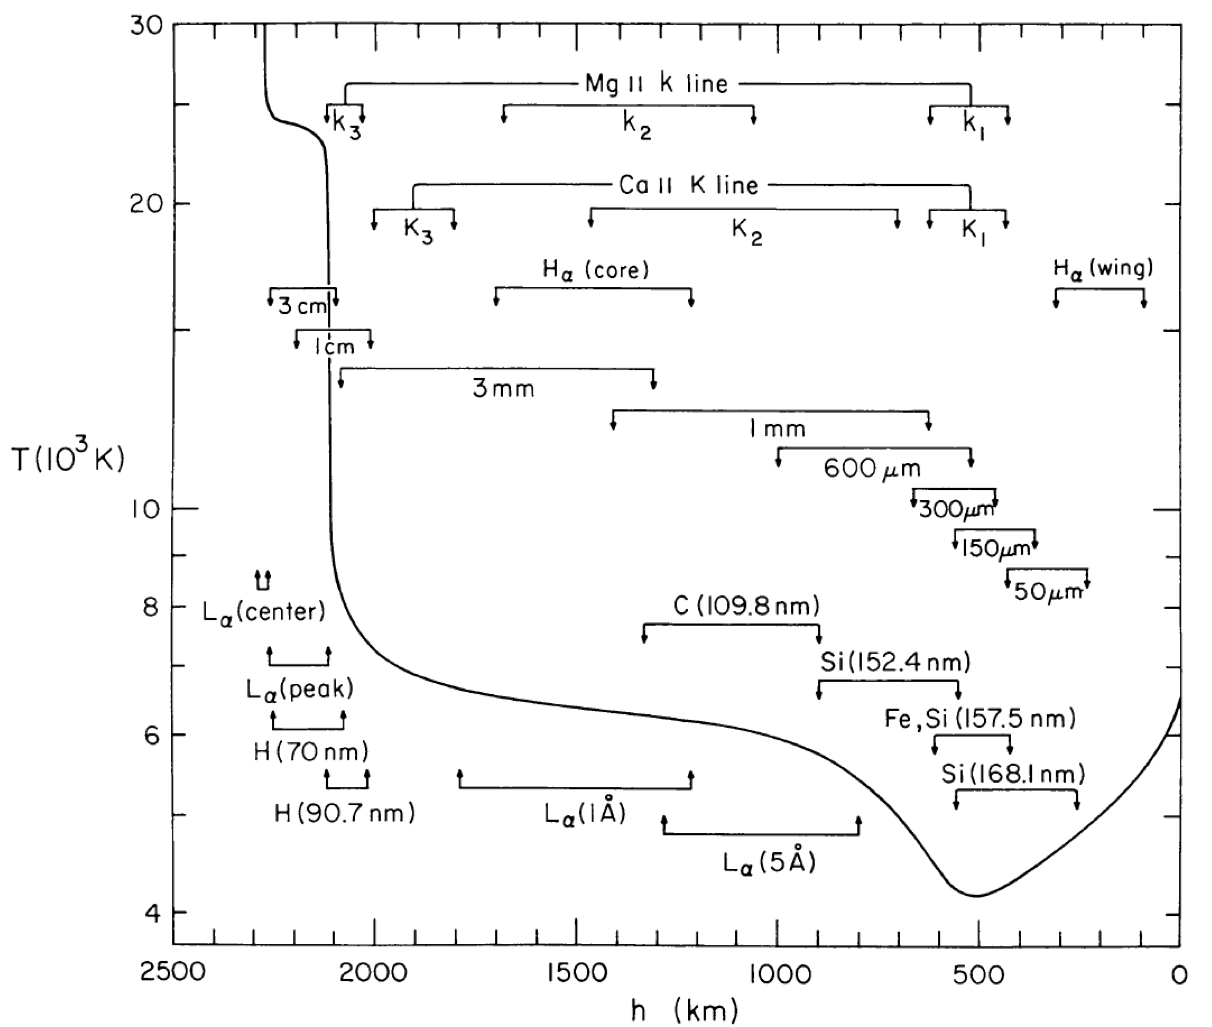
\includegraphics[width=0.95\linewidth]{figs/fig8}
	\caption{一些色球谱线和它们对应的形成高度。来源:\textcite{Vernazza1981}}
	\label{fig:8}
	\end{minipage}%
	\hfill
	\begin{minipage}[t]{0.5\linewidth}
	\centering
	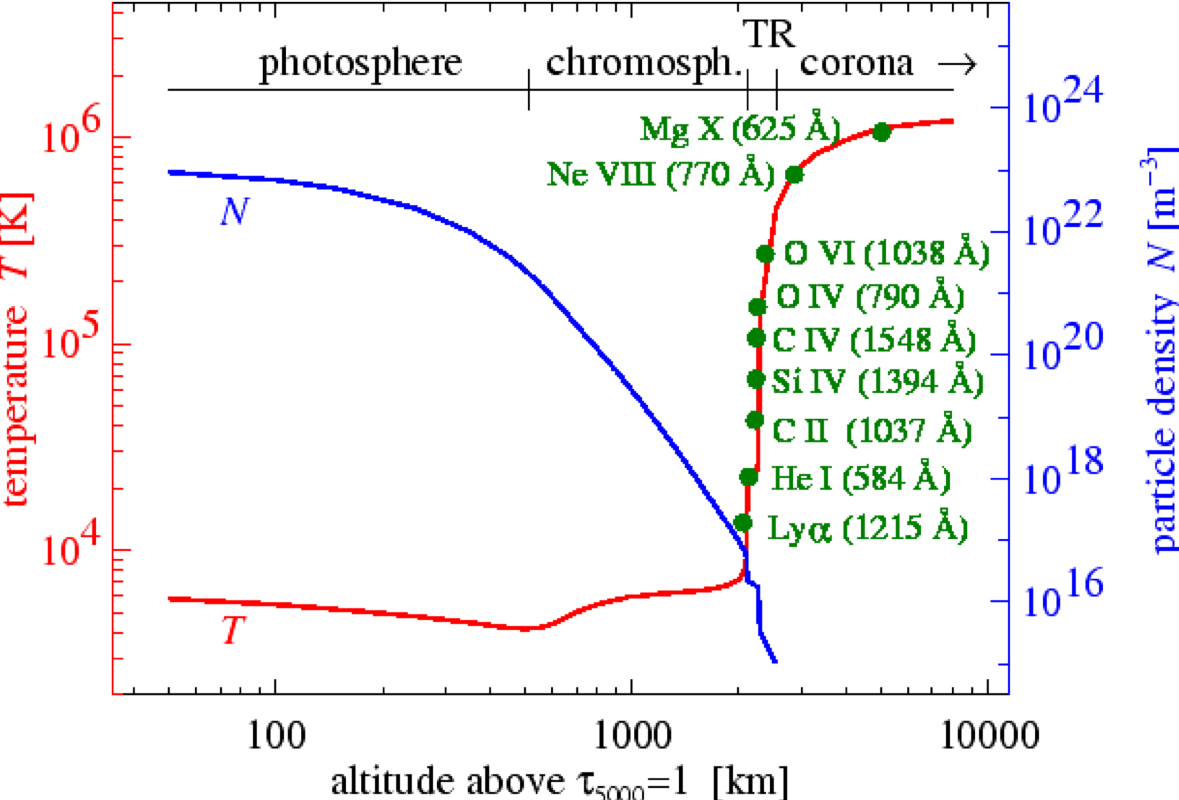
\includegraphics[width=0.95\linewidth]{figs/fig9}
	\caption{部分过渡区谱线和对应的形成高度。来源:\textcite{Peter2004}}
	\label{fig:9}
	\end{minipage}
\end{figure}
\subsection{Mg \textsc{ii}线}
Mg \textsc{ii}离子形成的发射/吸收线在UV波段较为明显的是Mg \textsc{ii} h, k和三重线。Mg \textsc{ii} h和k 线($\lambda_h = 2803.53~\mbox{\AA}, \lambda_k = 2796.35~\mbox{\AA}$,注意:在这篇文章中所有紫外谱线的波长都是真空波长)是太阳色球光谱中最明显的两条发射线之一。它们是Mg \textsc{ii}原子第一激发态到基态跃迁的共振线,由于第一激发态精细结构能级劈裂而分裂成两条,对应上下能级分别为从$3p\ ^2\mathrm{P}_{1/2}$到$3s\ ^2\mathrm{S}_{1/2}$和从$3p\ ^2\mathrm{P}_{3/2}$到$3s\ ^2\mathrm{S}_{1/2}$能级。在h和k线波长附近,还有另外三条谱线($\lambda = 2791.60~\mbox{\AA},\ 2798.75~\mbox{\AA}$ 和 $2798.82~\mbox{\AA}$),它们被称为三重线。在本文中波长较短的被称作Mg \textsc{ii} 2791线,而另外两条重叠的波长较长的线被称作Mg \textsc{ii} 2798线。它们来自于Mg \textsc{ii}第二激发态到第一激发态的跃迁,对应的能级分别为从$3d\ ^2\mathrm{D}_{3/2}$到$3p\ ^2\mathrm{P}_{1/2}$, $3d\ ^2\mathrm{D}_{3/2}$到$3p\ ^2\mathrm{P}_{3/2}$和从$3d\ ^2\mathrm{D}_{5/2}$到$3p\ ^2\mathrm{P}_{3/2}$。由于这些谱线都位于NUV波段,因此只能在离开地面足够高的高度进行观测。一些早期对宁静太阳上Mg \textsc{ii} h和k线的观测都显示了它们具有线心反转(\textit{central reversal})的结构\parencite{Lemaire1967,Lemaire1969,Doschek1977},而在耀斑带上则没有这样的结构,是一条纯发射线\parencite{Kohl1976K,Feldman1977}。一些辐射转移模拟也证明Mg \textsc{ii} h和k线的线心形成在高色球,而线翼则形成在低色球和温度极小区附近\parencite{Vernazza1981},见图~\ref{fig:8}。同时在NLTE的辐射转移模拟中,PRD效应被认为对Mg \textsc{ii} h和k线的形成起了重要作用,同时谱线的线心反转来自于线心形成与NLTE情况下,线心源函数在形成高度以下已经和Planck函数脱耦\parencite{Milkey1974,Ayres1976,Uitenbroek1997}。

在IRIS卫星发射前,针对其能观测到的一系列重要谱线(包括Mg \textsc{ii})在宁静太阳和谱斑等区域的谱线轮廓与形成高度进行了一系列的三维辐射磁流体力学模拟。在这一系列模拟中,再次确认了PRD效应对Mg \textsc{ii}谱线形成的重要性,且发现三维辐射转移对Mg \textsc{ii} h和k线的线心形成有比较重要的影响\parencites{Leenaarts2013a}。\textcites{Leenaarts2013b}进一步指出可以把Mg \textsc{ii} h和k线作为诊断太阳高层色球大气速度和温度的重要工具。\textcites{Pereira2015}研究了Mg \textsc{ii}三重线模拟中的谱线特征,他们发现大多数情况下Mg \textsc{ii}三重线形成与低色球并且是吸收线。但当低色球被加热时,Mg \textsc{ii}三重线会从吸收线转变为发射线,其线心线翼强度比可以用来推断低色球温度升高程度。

IRIS卫星发射后,观测到了一系列在耀斑带上轮廓出现明显变化的Mg \textsc{ii}线。Mg \textsc{ii} h,k包括三重线一般都显现出无线心反转的发射特征(见图\ref{fig:3})\parencites{Tian2015,Kerr2015,Tian2018}。Mg \textsc{ii} h和k线一般展现出较小的红翼不对称性和一个大约为十几$ \mathrm{km}\ \mathrm{s^{-1}}$的红移\parencites{Li2015,Li2017,Tian2018}。在一些比较大的耀斑中,IRIS卫星还在耀斑带的前缘发现了一些存在中心反转,但有着强烈红翼增强的Mg \textsc{ii} h和k线\parencites{Liu2015,Panos2018}。在某些耀斑爆发的初期,还观测到了一部分蓝翼增强的Mg \textsc{ii} h和k线,可能来自于一部分较冷物质$\sim10^4$ K在色球蒸发初期的上流\parencites{Tei2018}。

这些在宁静太阳上难以观测到的Mg \textsc{ii}谱线特征激发了新一轮的辐射流体力学模拟的兴趣,由于耀斑过程中的色球动力学过程非常复杂,这些模拟目前还只是在使用一维辐射流体力学代码(RADYN: \cites{Allred2005,Allred2015}; \cites{Carlsson1992,Carlsson1997}; RH: \cites{Uitenbroek2001}; \cites{Pereira2015b})进行计算。\textcites{Rubio2016}对2014年3月29日的X1.1级耀斑进行了模拟,他们发现耀斑带上的Mg \textsc{ii}线在模拟中仍然处于线心反转并且与观测相比显得非常窄。之后的一个参数研究工作通过人为提高Mg \textsc{ii}线心形成位置附近的电子密度一个量级,以保持LTE条件,在观测上再现了Mg \textsc{ii}非线心反转的谱线特征。但是这些合成的(\textit{synthetic})谱线仍然不够宽\parencites{Rubio2017}。同时\textcites{Rubio2017}提出一些剧烈增宽的非对称的谱线可以通过两个在观测上没有分辨的速度达到约$250\ \mathrm{km}\ \mathrm{s^{-1}}$速度上下流造成的红蓝移谱线叠加而成。另外一些通过对模拟得到的Mg \textsc{ii}谱线在时间上进行叠加的“多环”(\textit{multi-thread})模拟也能够部分再现Mg \textsc{ii}谱线的致宽和解释Doppler频移变化\parencites{Reep2019}。\textcites{Kerr2016}用Alfv\'en波加热低层大气来模拟耀斑能量释放,他们发现Mg \textsc{ii} h和k线逐渐由线心反转变为非线心反转,但谱线的红翼不对称性和致宽特征并没有得到很好的再现。


\subsection{Si \textsc{iv}线}
位于太阳光谱FUV波段的Si \textsc{iv}双重线($\lambda = 1393.755~\mbox{\AA}, 1402.770~\mbox{\AA}$)是Si \textsc{iv}的基态到第一激发态跃迁产生的两条共振线,由于原子能级精细结构分裂而形成两条线,对应的能级分别是从$2p^63s\ ^2\mathrm{S}_{1/2}$到$2p^63p\ ^2\mathrm{P}_{3/2}$与$2p^63s\ ^2\mathrm{S}_{1/2}$到$2p^63p\ ^2\mathrm{P}_{1/2}$。这两条线在70-80年代也在各类恒星,乃至类星体的光谱中被观测到\parencites{Stalio1975,Imhoff1980,Saxner1981,Oranje1982}。由于Si \textsc{iv}离子较高的电离态,其一般被认为是在过渡区温度约为$8\times10^4$ K处形成\parencites{Jordan1969,Doschek1997}。在太阳上对Si \textsc{iv}线的观测最早来自于\textcites{Brueckner1972,Brueckner1973}。在70年代末,天空实验室(\textit{Skylab}),环绕太阳天文台8(\textit{Orbiting Solar Observatory 8, OSO-8})和太阳极大年任务(\textit{Solar Maximum Mission, SMM})上搭载的光谱仪对宁静太阳\parencites{Doschek1976,Mariska1978,Shine1976}、冕洞\parencites{Feldman1976,Francis1977}、网状结构\parencites{Feldman1976b}和耀斑带上\parencites{Porter1984}等位置的Si \textsc{iv}线和其它紫外谱线分别从日面和临边角度进行了大量观测。由于一般认为它们在日面上是光学薄的(两条线发射强度比为2:1),且谱线形状能较好得被单Gaussian形的谱线拟合,所以被大量运用在测量运动速度\parencites{Feldman1976,Gebbie1981},湍动速度\parencites{Feldman1977c},建立过渡区模型\parencites{Roussel-Dupre1981}等研究。在临边高出2-4个角秒以上,Si \textsc{iv}的光学深度会明显增加,但通过一些简单的辐射转移近似也可以用来研究过渡区中的物质流动\parencites{Roussel-Dupre1979,Doschek1981}。

IRIS卫星发射后,Si \textsc{iv}线的观测又迎来了一个新的爆发式发展的时代。特别是针对一系列耀斑带的观测,Si \textsc{iv}线作为过渡区的重要发射线几乎在所有的耀斑观测中都得到了分析。在耀斑带上,Si \textsc{iv}往往展现出复杂的谱线形状。在一些耀斑中,Si \textsc{iv}仅出现强烈的红翼增强,但没有完全红移\parencites{Tian2014,Tian2015,Tian2018,Brosius2015,Polito2016},其中有一些谱线轮廓可以被一个红移较小的Gauss分量和另一个红移较大的Gauss分量拟合\parencites{Li2015,Lee2017}。而在另一些耀斑中,Si \textsc{iv}谱线又展现出一个整体红移约为$\sim50\ \mathrm{km}\ \mathrm{s^{-1}}$的单Gaussian形分量\parencites{LiD2017,Li2017},这可能来自于非热电子或热传导加热低层大气的高度和程度差异\parencites{Li2017}。和Mg \textsc{ii} h和k线的演化相比,这些红移/红翼不对称性一般会持续较长的时间\parencites{Warren2016},同时可能伴随着一个周期为0.5-6分钟的亮度准周期性振荡(\textit{quasi-periodic fluctuation}, \cites{Brosius2015,Zhang2016,Tian2018}),可能来自于日冕中的多次的重联过程\parencites{Brosius2015}。整个谱线的红移/红翼不对称性被普遍认为是存在较冷物质向下运动的重要证据,但对于其具体机制还存在着不同解释:\textcites{Reep2016}和~\textcites{Warren2016}认为其来自于多个耀斑环的持续的辐射冷却的叠加;\textcites{Tian2015}和~\textcites{Brannon2016}认为其来自于冷却的物质下流,还有认为其来自于较长的低层大气能量释放时间\parencites{Li2017}。

对耀斑带上Si \textsc{iv}谱线的辐射转移模拟较少,原因在于一般认为其是光学薄的,因此可以直接使用CHIANTI\parencites{Dere1997,Landi2013}等原子数据库进行计算。在耀斑带上观测到的明显的红翼不对称的谱线预示着Si \textsc{iv}线可能在耀斑带上存在光学厚的情况,需要细致的辐射转移计算。\textcites{Reep2016}在模拟中通过多个耀斑环叠加再现了Si \textsc{iv}谱线在耀斑带上的持续红移。\textcites{Kerr2019}利用RADYN代码对其进行了详细的辐射转移模拟,发现在较高非热电子能量加热($E>10^{10}\ \mathrm{erg}\ \mathrm{cm^{-2}s^{-1}}$)的耀斑中,形成于$3\times10^4-6\times10^4$ K间的Si \textsc{iv}线表现出光学厚的特征;而在较小的耀斑中($E<10^{10}\ \mathrm{erg}\ \mathrm{cm^{-2}s^{-1}}$),形成于$8\times10^4-10^5$ K间的Si \textsc{iv}线表现出光学薄的特征。
\subsection{C \textsc{ii}线}
在太阳FUV光谱中C \textsc{ii}线指在1335 \mbox{\AA}附近的三条谱线,是C \textsc{ii}离子第一激发态到基态的共振线,由于能级精细结构分裂成三条线($\lambda = 1334.532~\mbox{\AA}, 1335.663~\mbox{\AA}, 1335.708~\mbox{\AA}$),其中1335 \mbox{\AA}两条谱线由于波长相近而重叠在一起。它们对应的能级跃迁分别是从$2s^22p$ $^2\mathrm{P}_{1/2}$到$2s2p^2\ ^2\mathrm{D}_{3/2}$,$2s^22p\ ^2\mathrm{P}_{3/2}$到$2s2p^2\ ^2\mathrm{D}_{3/2}$与$2s^22p\ ^2\mathrm{P}_{3/2}$到$2s2p^2\ ^2\mathrm{D}_{5/2}$。\textcites{Detwiler1961}最早在太阳上观测到了FUV的C \textsc{ii}线,其谱线轮廓也在不久之后得到了准确的测量\parencites{Berger1970}。同时C \textsc{ii}线也在一系列的恒星中被观测到\parencites{Freire1979,Praderie1980,Kamp1982}。基于这些观测,\textcites{Berger1970}进行了一些基于统计平衡和NLTE的辐射转移计算,发现拟合较好的C \textsc{ii}线形成在$15000-20500$ K,宽度在$60-160$ Km的区域内。OSO-8卫星也对C \textsc{ii}谱线进行了一系列观测,其被发现对大气模型中的20000 K温度平台非常敏感\parencites{Lites1978},也被用于观测色球中波的传播\parencites{Chipman1978}。进一步的研究表明,活动区上的C \textsc{ii}总强度与活动区总磁通量有比较好的关系,可能是活动区中的磁力线对色球和日冕加热产生贡献导致的\parencites{Schrijver1987}。在耀斑发生时,C \textsc{ii}线强度也会剧烈增强,是FUV波段的连续谱的主要贡献之一\parencites{Doyle1992,Brekke1996}。

IRIS卫星的发射重新点燃了太阳物理学界对C \textsc{ii}线光谱诊断的兴趣。Rathore等人在2015年利用Bifrost三维辐射流体力学模拟的结果,深入探讨了各种因素对C \textsc{ii}在宁静太阳和谱斑区域的谱线形成的影响以及C \textsc{ii}作为光谱诊断工具的能力\parencites{Rathore2015a,Rathore2015b,Rathore2015c}。他们得到的结果包括:1)PRD效应对C \textsc{ii}谱线轮廓影响不大,但三维辐射转移效应对C \textsc{ii}线心形成起着重要作用。2)C \textsc{ii}线心大致形成在$6\times10^3-2.5\times10^4$ K间,对应的柱密度约为$10^6\ \mathrm{g}\ \mathrm{cm^{-2}}$的区域内。线心贡献函数最大处高度和过渡区高度(温度高于$3\times10^{4}$ K的最高高度)有非常好的相关性。3)光学深度对C \textsc{ii}谱线轮廓起着非常重要的作用,包括进一步致宽谱线和两条线的强度比。因此光谱诊断反演必须基于光学厚的辐射转移才能得到正确的结果。4)C \textsc{ii}线心在模拟中会存在单发射峰和线心反转(双峰)两种情况,线心反转谱线两个峰的不对称性和线心附近的大气速度梯度有关。5)谱线的Doppler频移能够比较好的反映线心形成高度的速度场。6)和形成在约为$8\times10^4$ K的Si \textsc{iv}线相比,C \textsc{ii}线和Mg \textsc{ii}线类似,都形成在相对较低的高度。C \textsc{ii}和Mg \textsc{ii}谱线的形成位置相对高低主要由$1.4\times10^4-5\times10^4$ K间物质密度分布决定。和IRIS观测到的谱线相比,他们的模拟也存在着一系列问题。其一是观测中的C \textsc{ii}线更宽,其半高全宽大约是模拟中的2倍;其二是模拟中的谱线大多是单发射峰,但观测上发现了大量的线心反转谱线,预示着C \textsc{ii}线心源函数在形成高度处也已经和Planck函数脱耦;其三是观测中C \textsc{ii}两线强度比(约为1.1-1.2)比模拟中得到的强度比(约1.4-1.7)要小。

在耀斑带上的C \textsc{ii}谱线也表现出类似于Mg \textsc{ii}和Si \textsc{iv}的轮廓结构,从有线心反转的谱线向单发射线转化,强度大约增强1-2个量级,谱线变宽,同时表现出一定的红翼不对称性\parencites{Li2015,Li2017}。C \textsc{ii}线的红移与Si \textsc{iv}线类似\parencites{Brosius2017},能够持续10分钟甚至更长的时间\parencites{Li2017}。在时间顺序上,C \textsc{ii}的红翼的增强出现于耀斑爆发相之前\parencites{Sadykov2015},也在IRIS能够观测到的高温谱线Fe XXI线在色球蒸发中出现明显蓝移之前\parencites{Brosius2018}。同时其红移大小在时间上与RHESSI卫星观测到的硬X射线12-25 KeV流量大小也有比较好的相关性\parencites{Sadykov2016}。在空间位置上,C \textsc{ii}的红移一开始也出现在耀斑带前缘\parencites{Battaglia2015},证明其与耀斑爆发中的非热电子入射或热传导有着比较强的关系。和Si \textsc{iv}线类似,耀斑带上的C \textsc{ii}线亮度也会产生准周期性的振荡\parencites{Brosius2015,Brosius2018},且其谱线宽度也会随着强度发生振荡\parencites{Warren2016}。此外在\textcites{Tei2018}中出现蓝移的Mg \textsc{ii}线位置上,C \textsc{ii}也展现了比较复杂的谱线轮廓,存在一个静止的存在线心反转的分量和一个比较强的红翼增强和不对称性。

\section{研究动机}
基于以上的研究我们可以看到,形成于色球和过渡区的紫外谱线对太阳以及M矮星上的各种各样的爆发活动均有不同程度的响应,为我们提供了获取这些爆发活动对应的色球和过渡区的动力学过程的重要诊断方法。但由于这些谱线大多形成在光学厚的区域,需要进行辐射转移的模拟才能理解其特征谱线轮廓对应的特定大气参数随高度的分布。在这篇论文中,我们将尝试使用已有的RADYN和RH代码,对这些不同的爆发时间都进行一定程度的研究。一方面我们希望检验这些代码在模拟这些不同尺度的爆发过程中的可用性和可靠性;另一方面我们也希望能够通过这些模拟帮助研究人员更好地理解在爆发过程中出现的特殊谱线轮廓究竟来自于哪些可能的物理过程。

% vim:ts=4:sw=4
